
\chapter{\hard\ 胀开}
\label{ch:blowing-up}

接下来我们讨论代数几何中的一个重要构造：沿一个闭子概形（由一个有限型理想层切出）\trBlowup{}一个概形。这套理论大体本可以在第 17 章之后立即展开；但对许多经典例子借助\trConormal{}锥／\trConormal{}丛／\trConormal{}层所作的诠释，使得把\trBlowup{}放在\trDifferential{}之后讨论显得顺理成章。

我们在后文不会太多用到\trBlowup，所以你现在大可跳过这个主题。但它是一件重要的工具。例如，可以用它来解消\trSingularPoint，更一般地，解消\trRationalMap{}的不定性。特别地，\trBlowup{}可用来把双有理的\trVariety{}彼此联系起来。

我们将从一个动机性的例子讲起，它会在一种特别重要（也是历史上最早）的情形中给你一幅构造的图像，见 \S22.1。然后我们会在 \S22.2 中看到用\trUniversalProperty{}表述的一个正式定义。这个定义与动机例子之间的联系并非一目了然。我们将从定义（假定\trBlowup{}确实存在）推出一些推论。然后在 \S22.3 中，我们将通过相当显式地描述\trBlowup，来证明\trBlowup{}存在。作为推论，我们会发现\trBlowup\trMorphism{}是射影的，并由此再推出更多的推论。在 \S22.4 中，我们将做一批显式计算，以见识各种应用，并看到许多事情都能徒手算出。


\section{动机例：胀开平面原点}

我们将推广下述概念，它将相应于仿射平面 $\mathbb{A}^2_k$ 原点的「\trBlowup」（\mbox{练习~10.3.F}）。我们的讨论将是非正式的。考虑 $\mathbb{A}^2\times\mathbb{P}^1$ 中相应于如下条件的子集。我们把 $\mathbb{P}^1$ 解读为过原点诸直线的参数化空间。考虑\trSubvariety
\[
\mathrm{Bl}_{(0,0)}\mathbb{A}^2:=\{(p\in\mathbb{A}^2,[\ell]\in\mathbb{P}^1)\;:\;p\in\ell\},
\]
它所给出的资料是：平面上的一个点 $p$，与一条同时包含 $p$ 和原点的直线 $\ell$。从代数上看：取 $x$、$y$ 为 $\mathbb{A}^2$ 上的\trCoordinate，$X$、$Y$ 为 $\mathbb{P}^1$ 上的射影\trCoordinate（与 $x$、$y$「相应」）；我们将考虑 $\mathbb{A}^2\times\mathbb{P}^1$ 中相应于 $xY-yX=0$ 的子集 $\mathrm{Bl}_{(0,0)}\mathbb{A}^2$。我们有一张有用的图：
\[
\begin{tikzcd}
\mathrm{Bl}_{(0,0)}\mathbb{A}^2\ar[r,hook]\ar[rd,"\beta"'] & \mathbb{A}^2\times\mathbb{P}^1\ar[r]\ar[d] & \mathbb{P}^1 \\
& \mathbb{A}^2 &
\end{tikzcd}
\]

你可以直接验证 $\mathrm{Bl}_{(0,0)}\mathbb{A}^2$ 在 $k$ 上\trSmooth{}（\mbox{定义~13.2.4}或\mbox{21.2.28}）（你现在可以让\mbox{练习~10.3.F}之后的那段话变得精确），但这里给出一个非正式的论证，利用\trProjection{} $\mathrm{Bl}_{(0,0)}\mathbb{A}^2\to\mathbb{P}^1$。\trProjectiveLine{} $\mathbb{P}^1$ 是\trSmooth{}的，而对于 $\mathbb{P}^1$ 中的每个点 $[\ell]$，直线 $\ell$ 上的诸点都有一个光滑的选取。这样，我们便是在通过 $\mathbb{P}^1$ 上的一个\trFibration{}来验证\trSmoothness。

接下来我们考虑投向 $\mathbb{A}^2$ 的\trProjection{} $\beta\colon\mathrm{Bl}_{(0,0)}\mathbb{A}^2\to\mathbb{A}^2$。它在原点之外是一个\trIsomorphism。粗略地说，若 $p$ 不是原点，则恰有一条直线同时包含 $p$ 和原点。另一方面，若 $p$ 就是原点，则同时包含 $p$ 和原点的直线有整整一个 $\mathbb{P}^1$ 那么多。于是 $(0,0)$ 的原像是一条\trCurve，从而是一个\trDivisor（一个\trEffectiveCartierDivisor，因为胀开所得的曲面是\trRegular{}的）。它称作这次\trBlowup{}的\trExceptionalDivisor。

倘若我们有一条在原点处\trSingular{}的\trCurve{} $C\subset\mathbb{A}^2$，那么借助这次\trBlowup，取 $C\setminus\{(0,0)\}$ 在 $\mathrm{Bl}_{(0,0)}\mathbb{A}^2$ 中的\trClosure，便有望把它部分地\trDesingularization。（一个\trVariety{} $X$ 的\textbf{\trDesingularization}（desingularization）或\textbf{\trResolutionOfSingularities}（resolution of singularities），是一个形如 $\widetilde{X}\to X$ 的\trProper{}\trBirational{}\trMorphism，其中 $\widetilde{X}$ 是\trRegular{}概形。）例如，考虑曲线 $y^2=x^3+x^2$，它除去原点处的一个\trNode{}之外处处\trRegular。我们可以取这条曲线去掉原点之后的原像，再取这一轨迹在\trBlowup{}中的闭包，便会得到一条正则曲线；结点在「楼下」的两个分支，到「楼上」就被分开了。（等到我们把各种概念恰当地定义好之后，你可以在\mbox{练习~22.4.B}中核验这件事。所得结果将称为这条曲线的\emph{\trProperTransform}（或称\emph{strict transform}，严格变换）。）我们出于许多理由关心\trDesingularization。由于我们对正则\trCurve{}的理解已经相当透彻，我们可望通过一条\trCurve{}的\trDesingularization{}来理解其他的曲线。这一哲学在高维情形同样成立。

更一般地，我们可以把 $\mathbb{A}^n$ 在原点处胀开（或者更不正式地说，「胀开原点」），得到 $\mathbb{A}^n\times\mathbb{P}^{n-1}$ 的一个\trSubvariety。从代数上看，若 $x_1,\dots,x_n$ 是 $\mathbb{A}^n$ 上的\trCoordinate，$X_1,\dots,X_n$ 是 $\mathbb{P}^{n-1}$ 上的射影\trCoordinate，则\trBlowup{} $\mathrm{Bl}_{\vec 0}\mathbb{A}^n$ 由诸方程 $x_iX_j-x_jX_i=0$ 给出。同样地，它是\trSmooth{}的：$\mathbb{P}^{n-1}$ 是\trSmooth{}的，而对于每个点 $[\ell]\in\mathbb{P}^{n-1}$，$p\in\ell$ 都有光滑的选取。

我们还可以更进一步：在上一个例子中添上 $m$ 个新变元 $x_{n+1},\dots,x_{n+m}$，从而把 $\mathbb{A}^{n+m}$ 沿一个坐标 $m$ 维平面 $\mathbb{A}^m$ 胀开；我们便得到 $\mathbb{A}^{n+m}\times\mathbb{P}^{n-1}$ 的一个子集。

由于在复几何中，\trManifold{}的子流形局部地「看起来像」$n$ 维空间中的坐标 $m$ 维平面，你或许会想象，我们可以把它推广为胀开正则\trVariety{}的正则\trSubvariety。在把这说精确的过程中，我们将意外地把这个概念大大推广，定义概形中任意\trFiniteType{}\trQC{}\trIdealSheaf{}的\trBlowup。一般而言，\trBlowup{}未必有「在正则之物内部胀开正则之物」那一情形下那样直观的描述——它可能对概形大施暴力——但即便如此，它仍然非常有用。

我们的描述将只依赖于被胀开的那个\trClosedSubscheme，而不依赖于坐标。这弥补了第一个例子——在原点处胀开平面——中本已存在的一个缺陷：倘若我们为平面选取不同的坐标（保持原点作为一个\trClosedSubscheme{}不变），我们并不会因此得到两个互不相同的胀开，这一点绝非显然。

一如常例，理解\trBlowup{}概念有两种方式，各有其适用的场合。第一种是通过\trUniversalProperty，它让你不费吹灰之力便能证出某些事情。第二种是显式构造，它让你亲手弄脏双手、把东西算出来（并且，比如说，蕴含了\trBlowup{}\trMorphism{}是\trProjective{}的这一事实）。

这里的动机例子也许看似一个非常特殊的情形，但只要你对 $n$ 维空间中原点的\trBlowup{}理解得足够透彻，你就会理解一般的\trBlowup。


\section{用泛性质胀开}

现在我们用\trUniversalProperty{}来定义\trBlowup。从这里讲起的不利之处在于：一眼看不出这个定义与 \S22.1 中的那些例子相同（甚至看不出它们有任何关系）。

设 $X\hookrightarrow Y$ 是一个\trClosedSubscheme，相应于某个\trFiniteType\trQC\trIdealSheaf。（若 $Y$ \trLocally\trNoetherian，则「\trFiniteType」这条假设自动成立，诺特读者尽可对它置之不理。）

$X\hookrightarrow Y$ 的\trBlowup{}是一个\trCartesianDiagram
\[
\tag{22.2.0.1}\label{eq:blowup-cartesian-diagram}
\begin{tikzcd}[row sep=3.2em, column sep=4.6em]
\mathrm{E}_X\,Y \ar[r,hook] \ar[d] & \mathrm{Bl}_X\,Y \ar[d,"\beta"'] \\
X \ar[r,hook] & Y
\end{tikzcd}
\]
使得 $\mathrm{E}_X\,Y$（$X$ 在 $\beta$ 之下的\trSchemeTheoreticPreimage）是 $\mathrm{Bl}_X\,Y$ 上的一个\trEffectiveCartierDivisor（定义于 \S9.5.1），使得其他任何一个这样的\trCartesianDiagram
\[
\tag{22.2.0.2}\label{eq:blowup-competing-diagram}
\begin{tikzcd}[row sep=3.2em, column sep=4.6em]
D \ar[r,hook] \ar[d] & W \ar[d] \\
X \ar[r,hook] & Y,
\end{tikzcd}
\]
其中 $D$ 是 $W$ 上的一个\trEffectiveCartierDivisor，都唯一地穿过它：
\[
\begin{tikzcd}[row sep=2.5em, column sep=4.2em]
D \ar[r,hook] \ar[d] & W \ar[d] \\
\mathrm{E}_X\,Y \ar[r,hook] \ar[d] & \mathrm{Bl}_X\,Y \ar[d] \\
X \ar[r,hook] & Y.
\end{tikzcd}
\]

我们称 $\mathrm{Bl}_X\,Y$ 为\textbf{\trBlowup}（沿 $X$ 对 $Y$ 胀开，或以 $X$ 为\textbf{\trCenter}（center）对 $Y$ 胀开）。（这项构造还有一些略显古旧的别名：\emph{单项变换}（monoidal transformation）、\emph{$\sigma$-过程}（$\sigma$-process）、\emph{二次变换}（quadratic transformation）与\emph{膨胀}（dilation）。）我们称 $\mathrm{E}_X\,Y$ 为这次\trBlowup{}的\trExceptionalDivisor。（$\mathrm{Bl}$ 与 $\beta$ 取自「blow-up（胀开）」，$\mathrm{E}$ 取自「exceptional（例外）」。）

（当心：在\trMinimalModelProgram（minimal model program）中，「\trExceptionalDivisor」的含义与此略有不同：若 $X\to Y$ 是一个\trBirational\trMorphism，则 $X$ 上任何一个在 $Y$ 中的像维数更低的\trWeilDivisor，在这种语境下也称作例外除子。）

由\trUniversalProperty{}的典型论证可知：若\trBlowup{}存在，则它在唯一\trIsomorphism{}的意义下唯一。（我们甚至可以借\trYonedaLemma{}的语言把它说得更显式：考虑由形如 \eqref{eq:blowup-competing-diagram} 的图组成的\trCategory，其中的\trMorphism{}是形如下图的资料
\[
\begin{tikzcd}[row sep=2.3em, column sep=2.7em]
D \ar[r,hook] \ar[drr] \ar[ddr] & W \ar[drr] \ar[ddr] & & \\
& & D' \ar[r,hook] \ar[dl] & W' \ar[dl] \\
& X \ar[r,hook] & Y. &
\end{tikzcd}
\]
那么\trBlowup{}就是这个\trCategory{}中的一个\trFinalObject——倘若它存在的话。）

若 $Z\hookrightarrow Y$ 是 $Y$ 的任一\trClosedSubscheme，则\trSchemeTheoreticPreimage{} $\beta^{-1}Z$ 称作 $Z$ 的\textbf{\trTotalTransform}（total transform）。我们很快会看到，$\beta$ 在离开 $X$ 的地方是一个\trIsomorphism（\mbox{观察~22.2.2}）。$\overline{\beta^{-1}(Z-X)}$ 则称作 $Z$ 的\textbf{\trProperTransform}、\textbf{严格变换}（strict transform）或\textbf{双有理变换}（birational transform）。（我们将采用第一个名称；后面还会在更一般的情形下定义它。）我们很快会看到（\mbox{\trBlowupClosureLemma~22.2.7}），\trProperTransform{}\trNaturalIsomorphism{}于 $\mathrm{Bl}_{Z\cap X}\,Z$，其中 $Z\cap X$ 是\trSchemeTheoretic{}交。

我们随后会证明\trBlowup{}总是存在，并把它显式地描述出来。首先我们来做一列观察——\emph{假定\trBlowup{}存在}。

\textbf{22.2.1.}\ \emph{观察。}\quad 若 $X$ 是空集，则 $\mathrm{Bl}_X\,Y=Y$。更一般地，若 $X$ 是一个\trEffectiveCartierDivisor，则\trBlowup{}是一个\trIsomorphism。（理由：$\id_Y\colon Y\to Y$ 满足这条\trUniversalProperty。）

\textbf{22.2.A.（练习）}\quad 若 $U$ 是 $Y$ 的一个\trOpenSubset，则 $\mathrm{Bl}_{U\cap X}\,U\cong\beta^{-1}(U)$，其中 $\beta\colon\mathrm{Bl}_X\,Y\to Y$ 是那个\trBlowup。

于是，「我们可以局部地计算\trBlowup。」

\textbf{22.2.B.（练习）}\quad 证明：若 $(Y_\alpha)$ 是 $Y$ 的一个\trOpenCover（$\alpha$ 跑遍某个\trIndexSet），而 $Y_\alpha$ 沿 $X\cap Y_\alpha$ 的\trBlowup{}存在，则 $Y$ 沿 $X$ 的\trBlowup{}存在。

\textbf{22.2.2.}\ \emph{观察。}\quad 把\mbox{观察~22.2.1} 与\mbox{练习~22.2.A} 结合起来便知：\trBlowup{}在你所胀开的轨迹之外是一个\trIsomorphism：
\[
\beta|_{\mathrm{Bl}_X\,Y\setminus\mathrm{E}_X\,Y}\colon \mathrm{Bl}_X\,Y\setminus\mathrm{E}_X\,Y \longrightarrow Y\setminus X
\]
是一个\trIsomorphism。

\textbf{22.2.3.}\ \emph{观察。}\quad 若 $X=Y$，则\trBlowup{}是空集：使得 $X$ 的拉回是一个\trEffectiveCartierDivisor{}的\trMorphism{} $W\to Y$ 唯有 $\varnothing\hookrightarrow Y$。这一下我们可就把 $Y$「胀没了」！

\textbf{22.2.C.（练习：\trBlowup{}保持\trIrreducibility{}与\trReducedness）}\quad 证明：若 $Y$ \trIrreducible，而 $X$ 不包含 $Y$ 的\trGenericPoint，则 $\mathrm{Bl}_X\,Y$ \trIrreducible。再证明：若 $Y$ \trReduced，则 $\mathrm{Bl}_X\,Y$ \trReduced。

\textbf{22.2.4. 首个非平凡情形中的存在性：胀开一个局部主闭子概形。}\quad
接下来我们来看为什么当 $X\hookrightarrow Y$ 局部地由一个方程切出时，$\mathrm{Bl}_X\,Y$ 存在。由于这个问题在 $Y$ 上是局部的（\mbox{练习~22.2.B}），我们化归到仿射情形 $\Spec A/(t)\hookrightarrow\Spec A$。（一个好例子是 $A=k[x,y]/(xy)$、$t=x$，值得把它想透。）令
\[
I=\ker(A\to A_t)=\{a\in A\;:\;t^na=0\ \text{对某个 } n>0\},
\]
并令 $\phi\colon A\to A/I$ 为\trProjection。

\textbf{22.2.D.（练习）}\quad 证明：$\phi(t)$ 在 $A/I$ 中不是\trZerodivisor。

\textbf{22.2.E.（练习）}\quad 证明：$\beta\colon\Spec A/I\to\Spec A$ 是 $\Spec A$ 沿 $\Spec A/t$ 的\trBlowup。换言之，证明
\[
\begin{tikzcd}[row sep=3em, column sep=5.4em]
\Spec A/(t,I) \ar[r] \ar[d] & \Spec A/I \ar[d,"\beta"'] \\
\Spec A/t \ar[r] & \Spec A
\end{tikzcd}
\]
是一个「胀开图」\eqref{eq:blowup-cartesian-diagram}。提示：在验证\trUniversalProperty{}时，先化归到 $W$（即 \eqref{eq:blowup-competing-diagram} 中的 $W$）为\trAffine{}的情形，再去解决由此产生的关于环的问题。视你的做法而定，你或许会觉得\mbox{练习~11.3.G}——它讲的是在\trEffectiveCartierDivisor{}之上\trMorphism{}延拓的唯一性——有帮助。

\textbf{22.2.F.（练习）}\quad 证明：$\Spec A/I$ 是 $D(t)$ 在 $\Spec A$ 中的\trSchemeTheoretic{}闭包。

于是你尽可以在几何上把 $\Spec A/I\to\Spec A$ 解读为「把支撑在 $V(t)$ 中的任何毛絮统统剃掉」。在诺特情形，这可以解读为删去那些落在 $V(t)$ 中的\trAssociatedPoint。这个说法本来就是刻意含糊的；只有当你自己想弄精确时，才需要去琢磨如何把它说精确。

\textbf{22.2.5. \trBlowupClosureLemma。}\quad
设有\trCartesianDiagram
\[
\begin{tikzcd}[row sep=3em, column sep=5.6em]
W \ar[r,hook,"\text{cl.~emb.}"'] \ar[d] & Z \ar[d] \\
X \ar[r,hook,"\text{cl.~emb.}"'] & Y,
\end{tikzcd}
\]
其中下面的那个\trClosedEmbedding{}相应于一个\trFiniteType\trIdealSheaf（从而上面的那个亦然）。头一遍读到这里时，只考虑 $Z\to Y$ 为\trClosedEmbedding{}的特殊情形，或许会有帮助。

然后把这个方块沿\trBlowup{} $\beta\colon\mathrm{Bl}_X\,Y\to Y$ 取\trFiberProduct，便得到\trFiberedCube（fibered cube）
\[
\tag{22.2.5.1}\label{eq:blowup-fibered-cube}
\begin{tikzcd}[row sep=2.2em, column sep=3.4em]
W\times_Y\mathrm{E}_X\,Y \ar[r,hook] \ar[d] \ar[ddr] & Z\times_Y\mathrm{Bl}_X\,Y \ar[d] \ar[ddr] \\
\mathrm{E}_X\,Y \ar[r,hook,"\text{Cartier}"'] \ar[ddr] & \mathrm{Bl}_X\,Y \ar[ddr] \\
& W \ar[r,hook,"\text{cl.~emb.}"'] \ar[d] & Z \ar[d] \\
& X \ar[r,hook,"\text{cl.~emb.}"'] & Y.
\end{tikzcd}
\]
其中顶部的方块正是\trCartesianDiagram
\[
\tag{22.2.5.2}\label{eq:blowup-top-square}
\begin{tikzcd}[row sep=3em, column sep=6.6em]
W\times_Y\mathrm{E}_X\,Y \ar[r,hook] \ar[d] & Z\times_Y\mathrm{Bl}_X\,Y \ar[d] \\
\mathrm{E}_X\,Y \ar[r,hook,"\text{Cartier}"'] & \mathrm{Bl}_X\,Y.
\end{tikzcd}
\]

\textbf{22.2.G.（简单练习）}\quad 为什么 \eqref{eq:blowup-top-square} 是一个\trCartesianDiagram？证明下面这批有用的\trCanonical{}同构：
\[
W\times_Y\mathrm{E}_X\,Y\cong Z\times_Y\mathrm{E}_X\,Y\cong W\times_Y\mathrm{Bl}_X\,Y.
\]

\textbf{22.2.6.}\quad \eqref{eq:blowup-top-square} 中下面的那个\trClosedEmbedding{}局部地由一个方程切出，于是上面的那个\trClosedEmbedding{}亦复如此。然而，$Z\times_Y\mathrm{Bl}_X\,Y$ 上的局部方程未必是\trNonZerodivisor，因而上面的\trClosedEmbedding{}未必是一个\trEffectiveCartierDivisor。

设 $\bar{Z}$ 为
\[
(Z\times_Y\mathrm{Bl}_X\,Y)\setminus(W\times_Y\mathrm{Bl}_X\,Y)
\]
在 $Z\times_Y\mathrm{Bl}_X\,Y$ 中的\trSchemeTheoretic{}闭包。（由于 $W\times_Y\mathrm{Bl}_X\,Y$ 是\trLocallyPrincipal{}的，我们恰好就处在 \S22.2.4 的情形之中，故这个\trSchemeTheoretic{}闭包并不神秘。）注意：在 $Z\to Y$ 为\trClosedEmbedding{}的特殊情形，$\bar{Z}$ 就是 \S22.2 中定义的\trProperTransform。有鉴于此，即便 $Z\to Y$ \emph{不}是\trClosedEmbedding，把 $\bar{Z}$ 称作 $Z$ 的\textbf{\trProperTransform}、把 $Z\times_Y\mathrm{Bl}_X\,Y$ 称作 $Z$ 的\textbf{\trTotalTransform}，也是合理的。

把 $\mathrm{E}_{\bar{Z}}\hookrightarrow\bar{Z}$ 定义为 $\mathrm{E}_X\,Y$ 拉回到 $\bar{Z}$ 上的结果，亦即由如下\trCartesianDiagram{}给出：
\[
\begin{tikzcd}[row sep=2.5em, column sep=5.2em]
\mathrm{E}_{\bar{Z}} \ar[r,hook] \ar[d,hook,"\text{cl.~emb.}"'] & \bar{Z} \ar[d,hook,"\text{cl.~emb.}"'] & \text{真变换} \\
W\times_Y\mathrm{E}_X\,Y \ar[r,hook,"\text{loc.~prin.}"'] \ar[d] & Z\times_Y\mathrm{Bl}_X\,Y \ar[d] & \text{\trTotalTransform} \\
\mathrm{E}_X\,Y \ar[r,hook,"\text{Cartier}"'] & \mathrm{Bl}_X\,Y. &
\end{tikzcd}
\]

注意，$\mathrm{E}_{\bar{Z}}$ 是 $\bar{Z}$ 上的一个\trEffectiveCartierDivisor。（它局部地由一个方程切出，而这个方程是把 $\mathrm{E}_X\,Y$ 在 $\mathrm{Bl}_X\,Y$ 上的某个局部方程拉回而来。你能看出为什么它在局部上不是\trZerodivisor{}吗？不妨注意：依据\mbox{练习~22.2.E} 与\mbox{练习~22.2.F}（外加\trBlowup{}可以仿射局部地计算这一事实），上图的顶部方块是一个胀开方块，这一点会有帮助。）

\textbf{22.2.7.\ \trBlowupClosureLemma。}\ ——\ \emph{沿用前述记号：$(\mathrm{Bl}_W\,Z,\ \mathrm{E}_W\,Z)$ \trCanonically\trIsomorphic{}于 $(\bar{Z},\ \mathrm{E}_{\bar{Z}})$。更精确地说：若\trBlowup{} $\mathrm{Bl}_X\,Y$ 存在，则 $(\bar{Z},\ \mathrm{E}_{\bar{Z}})$ 就是 $Z$ 沿 $W$ 的\trBlowup。}

这将会非常有用。我们先做几点初步评论。头三点适用于 $Z\to Y$ 为\trClosedEmbedding{}的特殊情形，而第四点评论基本上是在告诉我们：本不该把注意力都集中在这个特殊情形上。

（1）首先，注意若 $Z\to Y$ 是\trClosedEmbedding，则\mbox{\trBlowupClosureLemma}断言：\trProperTransform{}（如 \S22.2 中所定义）正是 $Z$ 沿\trSchemeTheoretic{}交 $W=X\cap Z$ 的\trBlowup。

（2）特别地，\mbox{\trBlowupClosureLemma}让你真能动手算出\trBlowup，我们很快就会做一大批例子。例如，设 $C$ 是一条平面\trCurve，在点 $p$ 处\trSingular，而我们想把 $C$ 在 $p$ 处胀开。那么我们可以转而把平面在 $p$ 处胀开（至于具体怎么做，我们已经描述过了，哪怕我们还未证明它满足胀开的\trUniversalProperty），然后再取 $C\setminus\{p\}$ 在这个\trBlowup{}中的\trSchemeTheoretic{}闭包。

（3）更一般地，若 $W$ 是某个我们想要胀开的讨厌子概形，而 $Z$ 是一个\trFiniteType{} $k$-\trScheme，则同样的技巧也能奏效。我们可以局部地工作（\mbox{练习~22.2.A}），故不妨假设 $Z$ \trAffine。若 $W$ 由 $r$ 个方程 $f_1,\dots,f_r\in\Gamma(Z,\OO_Z)$ 切出，则把这 $f$ 补全成 $\Gamma(Z,\OO_Z)$ 的一组生成元 $f_1,\dots,f_n$。这给出 $Z$ 向 $\mathbb{A}^n$ 中的一个\trClosedEmbedding，使得 $W$ 是 $Z$ 与一个坐标线性空间 $\mathbb{A}^{n-r}$ 的\trSchemeTheoretic{}交。

（4）还要更一般地，这把\trBlowup{}的存在性化归到了一个特定的特殊情形。（若你更愿意在固定的域 $k$ 上工作，尽可把这段讨论中的 $\mathbb{Z}$ 换成 $k$。）假设对每个 $n$，$\mathrm{Bl}_{V(x_1,\dots,x_n)}\Spec\mathbb{Z}[x_1,\dots,x_n]$ 都存在。那么我断言：\trBlowup{}总是存在。道理如下。我们不妨设 $Y$ \trAffine，比如说 $\Spec B$，而 $X=\Spec B/(f_1,\dots,f_n)$。于是我们有\trMorphism{} $Y\to\mathbb{A}^n_{\mathbb{Z}}$，它由 $x_i\mapsto f_i$ 给出，使得 $X$ 是原点的\trSchemeTheoreticPreimage。于是由\mbox{\trBlowupClosureLemma}，$\mathrm{Bl}_X\,Y$ 存在。（不过，我们并不会走这条路线。）

\textbf{22.2.H.（练习）}\quad 证明\mbox{\trBlowupClosureLemma~22.2.7}。提示：显然，应当用\trUniversalProperty{}来构造两个方向上的\trMorphism。构造下面这张图，也许有用，也许没用。（你会认出其中的底层立方体正是 \eqref{eq:blowup-fibered-cube}。）
\[
\begin{tikzcd}[row sep=1.7em, column sep=2.5em]
& \mathrm{E}_{\bar{Z}} \ar[rr,hook,"\text{eff.~Cartier}"] \ar[dl] \ar[dd,hook] & & \bar{Z} \ar[dl] \ar[dd,hook] \\
\mathrm{E}_W\,Z \ar[rr,hook,"\text{eff.~Cartier}"] \ar[dd] \ar[dr] & & \mathrm{Bl}_W\,Z \ar[dr] \ar[dd] & \\
& Z\times_Y\mathrm{E}_X\,Y \ar[rr,hook,"\text{loc.~prin.}"] \ar[dl] \ar[dd] & & Z\times_Y\mathrm{Bl}_X\,Y \ar[dl] \ar[dd] \\
W \ar[rr,hook] \ar[dd] & & Z \ar[dd] & \\
& \mathrm{E}_X\,Y \ar[rr,hook,"\text{eff.~Cartier}"] \ar[dl] & & \mathrm{Bl}_X\,Y \ar[dl] \\
X \ar[rr,hook] & & Y &
\end{tikzcd}
\]
钩形箭头表示\trClosedEmbedding；当这些\trMorphism{}进而还是\trLocallyPrincipal{}的、甚至是有效\trCartier{}除子时，图中也相应予以标注。\mbox{练习~11.3.G}（关于在\trEffectiveCartierDivisor{}之上\trMorphism{}延拓的唯一性）也许有用，也许没用。注意：若 $Z\to Y$ 实际上是\trClosedEmbedding，则 $Z\times_Y\mathrm{Bl}_X\,Y\to\mathrm{Bl}_X\,Y$ 亦然，从而 $\bar{Z}\to\mathrm{Bl}_X\,Y$ 也是如此。


\section{胀开存在且射影}

\textbf{22.3.1.}\quad 现在是时候证明\trBlowup{}总是存在的了。我们将看到两种论证，它们各有各的启发。二者都将推出\trBlowup{}\trMorphism{}是\trProjective{}的，从而是\trQuasicompact、\trProper、\trFiniteType{}且\trSeparated{}的。特别地，若 $Y\to Z$ \trQuasicompact（相应地，\trProper、\trFiniteType、\trSeparated），则 $\mathrm{Bl}_X\,Y\to Z$ 亦复如是。（又若 $Y\to Z$ \trProjective{}而 $Z$ \trQuasicompact，则 $\mathrm{Bl}_X\,Y\to Z$ \trProjective。至于这条恼人的附加假设缘何出现，参看\mbox{练习~17.3.I} 的解答。）$k$-\trVariety{}的\trBlowup{}是 $k$-\trVariety（利用\trReducedness{}被保持这一事实，\mbox{练习~22.2.C}），而\trIrreducible{} $k$-\trVariety{}的\trBlowup{}是\trIrreducible{}的 $k$-\trVariety（利用\trIrreducibility{}被保持这一事实，同样见\mbox{练习~22.2.C}）。

\textbf{22.3.2. \trhTheorem（胀开的 $\mathit{Proj}$ 描述）。}\ ——\ \emph{设 $X\hookrightarrow Y$ 是由一个\trFiniteType\trQC\trIdealSheaf{} $\mathscr{I}\hookrightarrow\OO_Y$ 切出的\trClosedSubscheme。则}
\[
\mathit{Proj}_Y\bigl(\OO_Y\oplus\mathscr{I}\oplus\mathscr{I}^2\oplus\mathscr{I}^3\oplus\cdots\bigr)\longrightarrow Y
\]
\emph{满足胀开的\trUniversalProperty。}

（我们在\mbox{练习~15.6.E} 中赋予了\trIdealSheaf{}之乘积、从而 $\mathscr{I}^n$ 的意义。）
我们很快就会证明\mbox{定理~22.3.2}（\S22.3.3），不过先来看看它告诉了我们什么。由于 $\mathscr{I}$ 是有限型的，这个\trSheafOfGradedAlgebras{}的次数 $1$ 分片是有限型的。这个\trSheafOfGradedAlgebras{}显然也在次数 $1$ 处生成。于是这个\trSheafOfAlgebras{}满足\mbox{假设~17.2.1}（「在次数 $1$ 处有限生成」）。

但首先，我们应当确认 $X$ 的原像确实是一个\trEffectiveCartierDivisor。我们可以仿射局部地工作（\mbox{练习~22.2.A}），故不妨设 $Y=\Spec B$，而 $X$ 由有限生成的\trIdeal{} $I$ 切出。于是
\[
\mathrm{Bl}_X\,Y=\mathit{Proj}_B\bigl(B\oplus I\oplus I^2\oplus\cdots\bigr).
\]
我们稍稍滥用了记号：使用 $\mathrm{Bl}_X\,Y$ 这个记号，是因为我们尚未证明它满足\trUniversalProperty。回想（\S13.9.1），\trGradedRing{} $B\oplus I\oplus\cdots$——记作 $B(I)_\bullet$——称为 $B$ 中\trIdeal{} $I$ 的\trRees{}代数。

$X$ 的原像可不是随随便便一个\trEffectiveCartierDivisor{}就够了；它相应于这个 $\mathit{Proj}$ 上的\trInvertibleSheaf{} $\OO(1)$。的确，$\OO(1)$ 相应于如下操作：取我们的\trGradedRing，砍掉最底下的分片，再把全部分次片向左滑动 $1$ 位（\S15.1.4）；它就是相应于分次模
\[
IB(I)_\bullet=I\oplus I^2\oplus I^3\oplus\cdots
\]
（其中第一个直加项 $I$ 的分次为 $0$）的那个\trInvertibleSheaf。但它也可以被解读为 $X$ 的\trSchemeTheoreticPreimage，后者相应于 $B$ 的\trIdeal{} $I$：
\[
IB(I)_\bullet=I\bigl(B\oplus I\oplus I^2\oplus\cdots\bigr)\hookrightarrow B\oplus I\oplus I^2\oplus\cdots=B(I)_\bullet.
\]

于是，$X\hookrightarrow Y$ 在
\[
\mathit{Proj}\bigl(\OO_Y(\mathscr{I})_\bullet\bigr)=\mathit{Proj}\bigl(\OO_Y\oplus\mathscr{I}\oplus\mathscr{I}^2\oplus\cdots\bigr)
\]
中的\trSchemeTheoreticPreimage——它相应于 $\mathscr{I}\OO_Y(\mathscr{I})_\bullet=\mathscr{I}\oplus\mathscr{I}^2\oplus\mathscr{I}^3\oplus\cdots$ 所相应的那个\trIdealSheaf——是类 $\OO(1)$ 的一个\trEffectiveCartierDivisor。一旦我们验证了这套构造确实给出\trBlowup，这个除子就将是我们那个\trExceptionalDivisor{} $\mathrm{E}_X\,Y$。

此外，我们看到\trExceptionalDivisor{}可以被漂亮地描述为 $X$ 上的一个 $\mathit{Proj}$：
\[
\tag{22.3.2.1}\label{eq:exceptional-divisor-proj}
\mathrm{E}_X\,Y=\mathit{Proj}_X\bigl(\OO_Y/\mathscr{I}\oplus\mathscr{I}/\mathscr{I}^2\oplus\mathscr{I}^2/\mathscr{I}^3\oplus\cdots\bigr)=\mathit{Proj}_X\bigl(\OO_Y(\mathscr{I})_\bullet/(\mathscr{I}\OO_Y(\mathscr{I})_\bullet)\bigr).
\]
日后我们会看到，在好的境况下（若 $X$ 是 $Y$ 中的\trRegularEmbedding），这是某个\trVectorBundle{}的射影化（「\trProjectivization\trNormalBundle」）；见\mbox{练习~22.3.D}(a)。

\textbf{22.3.3. \mbox{定理~22.3.2} 的证明。}\quad 化归到仿射靶 $Y=\Spec B$（$X$ 相应于\trIdeal{} $I\subset B$）的情形。再化归到仿射源 $\Spec R$（带主\trEffectiveCartierDivisor{} $V(t)$，$t$ 是 $R$ 中的\trNonZerodivisor）的情形。（一个主\trEffectiveCartierDivisor{}局部地由单个\trNonZerodivisor{}切出。）于是我们化归到了 $\pi\colon\Spec R\to\Spec B$（相应于 $\phi\colon B\to R$）的情形。选取 $x_1,\dots,x_n$，使得 $(x_1,\dots,x_n)=I$，且 $(\phi(x_1),\dots,\phi(x_n))=(t)$。（这里我们用到了「$V(I)$ 的概形论拉回是 $V(t)$」这条假设，以及\mbox{练习~10.2.B} 对概形论拉回的理解。）从而
\[
\tag{22.3.3.1}\label{eq:phin-generated-unit}
(\phi(x_1)/t,\dots,\phi(x_n)/t)=R.
\]
（因为 $t$ 是\trNonZerodivisor，$\phi(x_i)/t$ 是有意义的。）我们将描述\emph{一个}映射 $\Spec R\to\Proj B(I)_\bullet$，它将把\trOpenSet{}上的那个映射 $\Spec R_t\to\Spec B$ 延拓开来。而由\mbox{练习~11.3.G}，它便是唯一的。考虑环映射 $\phi'\colon B(I)_\bullet\to R$，它把次数为 $d$ 的元素 $X$ 送到 $\phi(X)/t^d$。这就诱导出从 $\Spec R$ 到\textbf{\trAffine\trCone}（affine cone）$\Spec B(I)_\bullet$ 的一个映射 $\pi'$。

令 $X_i$ 为 $B(I)_\bullet$ 中相应于 $x_i$ 的次数 $1$ 元素。于是 $\phi'$ 诱导出
\[
\bigl((B(I)_\bullet)_{X_i}\bigr)_0\longrightarrow R_{\phi(x_i)/t},
\]
从而在几何上诱导出 $\mathrm{D}(\phi(x_i)/t)\to\mathrm{D}(X_i)$：从 $\Spec R$ 的一个\trDistinguishedOpen{}到\trAffine\trCone $\Spec B(I)_\bullet$ 的一个\trDistinguishedOpen。当 $x$ 跑遍集合 $\{x_1,\dots,x_n\}$ 时，诸 $\mathrm{D}(\phi(x_i)/t)$ 便跑遍 $\Spec R$ 的一组特异开覆盖（由 \eqref{eq:phin-generated-unit}）。于是，$\pi'\colon\Spec R\to\Spec B(I)_\bullet$ 的像避开\trIrrelevantIdeal{} $(X_1,\dots,X_n)\subset B(I)_\bullet$ 的\trVanishingSet，故映射 $\pi'$ 穿过 $\Spec B(I)_\bullet\setminus V(X_1,\dots,X_n)$，从而映入 $\Proj B(I)_\bullet$（一切都与到 $\Spec B$ 的态射交换）：
\[
\begin{tikzcd}[row sep=2.8em, column sep=3.4em]
\Spec B(I)_\bullet & \Spec B(I)_\bullet\setminus V(X_1,\dots,X_n) \ar[l,hook] \ar[r] \ar[d] & \Proj B(I)_\bullet \ar[dl] \\
\Spec R \ar[u,"\pi'"] \ar[ur,dotted] \ar[r,"\pi"] & \Spec B &
\end{tikzcd}
\]
我们便构造出了想要的态射 $\Spec R\to\Proj B(I)_\bullet$，它「提升」$\pi$。\hfill$\square$

以下是由这套\trBlowup{}构造派生的一些应用与观察。首先，我们可以验证，最初那批动机例子确实是胀开。例如，在原点处胀开 $\mathbb{A}^2$（带\trCoordinate{} $x$、$y$）给出：$B=k[x,y]$、$I=(x,y)$，而 $\Proj(B\oplus I\oplus I^2\oplus\cdots)=\Proj B[X,Y]$，其中 $B$ 的元素次数为 $0$，而 $X$ 与 $Y$ 的次数为 $1$，且分别与 $x$、$y$「相应」。

\textbf{22.3.4.}\ \emph{\trExceptionalDivisor{}的\trNormalBundle。}\quad 一个\trEffectiveCartierDivisor{} $D$ 的\trNormalBundle，就是（与）\trInvertibleSheaf{} $\OO(D)|_D$ 相伴随的空间——$\OO(D)$ 是\trTotalSpace{}上相应于 $D$ 的那个\trInvertibleSheaf，再限制到 $D$ 上（\mbox{练习~21.2.J}）。于是，在平面内一点处胀开的情形，\trExceptionalDivisor{}的\trNormalBundle{}是 $\OO(-1)$。（插一句：\trCastelnuovo{}判别准则（\mbox{定理~28.6.1}）断言其逆：给定一个光滑\trSurface，若它含有满足 $E\cong\mathbb{P}^1$ 且\trNormalBundle{}为 $\OO(-1)$ 的 $E$，则 $E$ 可以被收缩成另一个光滑\trSurface{}上的一点。）在正则\trVariety{}的正则\trSubvariety{}之胀开的情形，胀开结果是正则的（见\mbox{定理~22.3.10}），\trExceptionalDivisor{}是 $X$ 上的一个射影丛，而\trExceptionalDivisor{}的\trNormalBundle{}限制为 $\OO(-1)$（\mbox{练习~22.3.D}）。

\textbf{22.3.A.（较难而富启发的练习）}\quad 设 $\iota\colon X\hookrightarrow\mathbb{P}^n$ 是一个\trProjective\trScheme，请把 $X$ 上的\trAffine\trCone（\S9.3.11）在原点处的\trBlowup{}的\trExceptionalDivisor{}与 $X$ 本身等同起来，并证明它的\trNormalBundle（\S22.3.4）\trIsomorphic{}于 $\OO_X(-1):=\iota^*\OO_{\mathbb{P}^n}(-1)$。（在 $X=\mathbb{P}^1$ 的情形，我们便重新得到了平面在一点处的胀开。特别地，我们重新得到了那条重要事实：\trExceptionalDivisor{}的\trNormalBundle{}是 $\OO(-1)$。）

\textbf{22.3.5.}\ \emph{\trNormal\trCone。}\quad 受 \eqref{eq:exceptional-divisor-proj} 以及下方\mbox{练习~22.3.D} 的激励，我们给出如下定义。若 $X$ 是 $Y$ 中由 $\mathscr{I}$ 切出的\trClosedSubscheme，则 $X$ 在 $Y$ 中的\textbf{\trNormal\trCone}（normal cone）$\mathrm{N}_X\,Y$ 定义为
\[
\tag{22.3.5.1}\label{eq:normal-cone}
\mathrm{N}_X\,Y:=\mathit{Spec}_X\bigl(\OO_Y/\mathscr{I}\oplus\mathscr{I}/\mathscr{I}^2\oplus\mathscr{I}^2/\mathscr{I}^3\oplus\cdots\bigr).
\]
这可以卓有成效地解读为无穷小「\trTubularNeighborhood」的一种代数几何版本。但有几点当心事项。若 $Y$ \trSmooth，$\mathrm{N}_X\,Y$ 未必\trSmooth。（你可以自己算一算 $Y=\mathbb{A}^2_k$、$X=V(xy)$ 这个例子。）

而且即便 $X$ 与 $Y$ 都\trSmooth，虽然 $\mathrm{N}_X\,Y$ 是\trSmooth{}的（我们稍后就会看到，\mbox{练习~22.3.D}），它却无论如何也不「嵌入」到 $Y$ 之中。举一个简单的例子：考虑非有理\trCurve{} $Y=C$ 的一个\trSmooth{}点 $X=p$。那么 $\mathrm{N}_X\,Y$ 是有理的，从而不可能开嵌入到 $Y$ 中。

\textbf{22.3.6.}\ \emph{\trTangent\trCone。}\quad 若 $X$ 是一个\trClosedPoint{} $p$，则\trNormal\trCone{}称作 $Y$ 在 $p$ 处的\textbf{\trTangent\trCone}（tangent cone）。\textbf{\trProjectivization\trTangent\trCone}（projectivized tangent cone）则是\trExceptionalDivisor{} $\mathrm{E}_X\,Y$（同一个\trSheafOfGradedAlgebras{}的 $\mathit{Proj}$）。沿循 \S9.3.12，\trTangent\trCone{}与\trProjectivization\trTangent\trCone{}可以拼合到\trTangent\trCone{}的\trProjectiveCompletion{}之中：后者包含\trTangent\trCone{}作为\trOpenSubset，并包含\trProjectivization\trTangent\trCone{}作为互补的\trEffectiveCartierDivisor。

在\mbox{练习~22.3.D} 中我们将看到：在 $Y$ 的正则点处，\trTangent\trCone{}可以与\trTangentSpace{}等同起来，而\trNormal\trCone{}往往可以与\trNormalBundle{}的\trTotalSpace{}等同起来。

\textbf{22.3.B.（练习）}\quad 设 $Y=\Spec k[x,y]/(y^2-x^2-x^3)$（\trNode{}三次曲线；见图~\ref{fig:normalization-nodal-cubic} 的底部）。假设（以免分心）$\operatorname{char}k\neq 2$。证明：$Y$ 在原点处的\trTangent\trCone\trIsomorphic{}于 $\Spec k[x,y]/(y^2-x^2)$。于是，不严格地说，\trTangent\trCone「看起来就像」原本那个\trVariety{}被「无穷放大」了。

\textbf{22.3.C.（练习）}\quad 设 $S_\bullet$ 是域 $k$ 上一个\trFinitelyGenerated{}的\trGradedAlgebra。\mbox{练习~22.3.A} 给出了 $\Proj S_\bullet$ 与「$\Spec S_\bullet$ 在原点处的胀开」的\trExceptionalDivisor{}之间的一个\trIsomorphism。证明：$\Spec S_\bullet$ 在原点处的\trTangent\trCone\trIsomorphic{}于 $\Spec S_\bullet$ 本身。（你的几何直觉应当会使你觉得这些事实可信。）

\textbf{22.3.7. 沿正则嵌入胀开。}\quad 对正则嵌入 $X\subset Y$ 作胀开，这一情形特别令人愉悦。例如，\trExceptionalDivisor{}是 $X$ 上的一个射影丛。

\textbf{22.3.8. \trhTheorem。}\ ——\ \emph{若 $I\subset A$ 由一个\trRegularSequence{} $a_1,\dots,a_d$ 生成，则自然映射 $\Sym^n_A(I/I^2)\to I^n/I^{n+1}$ 是一个\trIsomorphism。}

\textbf{22.3.9. \trhCorollary。}\ ——\ \emph{若\trClosedEmbedding{} $\iota\colon X\hookrightarrow Y$ 是带\trIdealSheaf{} $\mathscr{I}\subset\OO_Y$ 的一个\trRegularEmbedding，则自然映射 $\Sym^n(\mathscr{I}/\mathscr{I}^2)\to\mathscr{I}^n/\mathscr{I}^{n+1}$ 是一个\trIsomorphism。此外，结合\mbox{命题~21.2.16}，我们看到 $\mathscr{I}^n/\mathscr{I}^{n+1}$ 是一个\trLocallyFreeSheaf。}

\mbox{练习~24.6.E} 在 $A$ 是 $k$-代数的情形给出了\mbox{定理~22.3.8}（以及\mbox{推论~22.3.9}）的一个稍显简单的证明。

在 \S22.3.11 开始\mbox{定理~22.3.8} 的证明之前，我们先展示它的用处。

\textbf{22.3.D.（练习）}\quad
（a）设 $X\to Y$ 是带\trIdealSheaf{} $\mathscr{I}$ 的一个\trRegularEmbedding。请把正规层（「正规丛」）的\trTotalSpace（\S17.1.5）与\trNormal\trCone $\mathrm{N}_X\,Y$（\eqref{eq:normal-cone}）等同起来，并证明\trExceptionalDivisor{} $\mathrm{E}_X\,Y$ 是 $X$ 上的一个射影丛（「\trProjectivization\trNormalBundle」）。

（b）证明：$\mathrm{E}_X\,Y$ 在 $\mathrm{Bl}_X\,Y$ 中的\trNormalBundle{}是 $\OO(-1)$（对这个 $X$ 上的射影丛而言）。

（c）再设 $X$ 是一个\trReduced{}的\trClosedPoint{} $p$。证明：$p$ 是 $Y$ 的一个正则点。请把 $p$ 的\trTangentSpace{}的\trTotalSpace{}与 $Y$ 在 $p$ 处的\trTangent\trCone{}等同起来。

\textbf{22.3.10. \trhTheorem。}\ ——\ \emph{设 $X\hookrightarrow Y$ 是 $k$ 上光滑\trVariety{}之间的一个\trClosedEmbedding。则 $\mathrm{Bl}_X\,Y$ 也是\trSmooth{}的。}

\emph{证明。}\quad 我们用到「光滑\trVariety{}是正则的」，此即\mbox{光滑性--正则性比较定理~13.2.7}(b)——其证明尚待完成。

我们不妨设 $k=\overline{k}$，因为把结论作\trBaseChange{}到\trAlgebraicClosure{}后依然成立。理由：\trSmoothness{}可以在\trBaseChange{}到 $\overline{k}$ 之后检验，\mbox{练习~13.2.H}。胀开构造与到\trAlgebraicClosure{}的\trBaseChange{}交换：你可以直接审视这个构造，或者等到能够援引\mbox{练习~24.1.P}(a) 中的推广。

由\mbox{观察~22.2.2}，只须检验 $\mathrm{Bl}_X\,Y$ 在 $\mathrm{E}_X\,Y$ 的诸点处的\trSmoothness。由\mbox{练习~13.2.M}(b)，$X\hookrightarrow Y$ 是一个\trRegularEmbedding。那么由\mbox{练习~22.3.D}(a)，$\mathrm{E}_X\,Y$ 是 $X$ 上的一个射影丛，从而是\trSmooth{}的，进而在其\trClosedPoint{}处正则。但 $\mathrm{E}_X\,Y$ 是 $\mathrm{Bl}_X\,Y$ 上的一个\trEffectiveCartierDivisor。于是由正则性的\trSlicing{}判别法（\mbox{练习~13.2.C}），$\mathrm{Bl}_X\,Y$ 在 $\mathrm{E}_X\,Y$ 的诸\trClosedPoint{}处正则，从而在 $\mathrm{E}_X\,Y$ 的一切点处\trSmooth。\hfill$\square$

\textbf{22.3.11.}\ \hard\ \emph{\mbox{定理~22.3.8} 的证明。}\quad 头一遍阅读时，把\mbox{定理~22.3.8} 的证明跳过去也完全合理。我们对\mbox{定理~22.3.8} 的证明沿循 [F2, A.6.1]，而后者又沿循 [Dav]。证明将在 \S22.3.13 完成。首先，令 $\alpha$ 为\trGradedRing{}之间的映射
\[
\alpha\colon (A/I)[X_1,\dots,X_d]\longrightarrow\oplus_{n=0}^{\infty}I^n/I^{n+1},
\]
它把 $X_i$ 送到 $a_i$ 在 $I/I^2$ 中的像。显然，$\alpha$ 是\trSurjectiveMap。

\textbf{22.3.E.（练习）}\quad 证明：\mbox{定理~22.3.8} 将由「$\alpha$ 是一个\trIsomorphism」这条陈述推出。

由于 $a_1$ 是\trNonZerodivisor，我们可以把 $A[a_2/a_1,\dots,a_d/a_1]$ 解读为\trTotalFractionRing（定义于 \S6.6.35）的一个子环。特别地，由于 $A$ 是其全分式环的子环，映射 $A\to A[a_2/a_1,\dots,a_d/a_1]$ 是\trInjectiveMap。定义
\[
\beta\colon A[T_2,\dots,T_d]\longrightarrow A[a_2/a_1,\dots,a_d/a_1]
\]
为 $T_i\mapsto a_i/a_1$。显然，映射 $\beta$ 是\trSurjectiveMap，而 $L_i:=a_1T_i-a_i$ 落在 $\ker(\beta)$ 之中。

\textbf{22.3.12. \trhLemma。}\ ——\ \emph{$\beta$ 的\trKernel{}是 $(L_2,\dots,L_d)$。}

\emph{证明。}\quad 我们对 $d$ 作归纳来证明这条结果。先考虑基底情形 $d=2$。设 $F(T_2)\in\ker\beta$，于是 $F(a_2/a_1)=0$。然后应用\trRemainderTheorem（Remainder Theorem）的算法，把 $a_1^{\deg F}F(T_2)$ 除以 $a_1T_2-a_2=L_2$，得
\[
\tag{22.3.12.1}\label{eq:division-remainder}
a_1^{\deg F}F(T_2)=G(T_2)(a_1T_2-a_2)+R,
\]
其中 $G(T_2)\in A[T_2]$，而 $R\in A$ 是余项。代入 $T_2=a_2/a_1$（并用「$A\to A[a_2/a_1]$ 为\trInjectiveMap」这一事实），便得 $R=0$。于是 $(a_1T_2-a_2)G(T_2)\equiv 0\pmod{(a_1^{\deg F})}$。利用「$a_2$ 模 $(a_1^{\deg F})$ 是\trNonZerodivisor」这一事实（因为 $a_1^{\deg F},a_2$ 是一个\trRegularSequence，\mbox{练习~9.5.E}），一次短归纳便表明 $G(T_2)$ 的系数必全被 $a_1^{\deg F}$ 整除。于是 $F(T_2)$ 被 $a_1T_2-a_2=L_2$ 整除，故 $d=2$ 的情形得证。

现在考虑一般情形 $d>2$，假定结果对一切更小的 $d$ 成立。令 $A'=A[a_2/a_1]$。那么 $a_1,a_3,a_4,\dots,a_d$ 是 $A'$ 中的一个\trRegularSequence。理由：$a_1$ 是 $A'$ 中的\trNonZerodivisor。$A'/(a_1)=(A[T_2]/(a_1T_2-a_2))/(a_1)=A[T_2]/(a_1T_2-a_2,a_1)=A[T_2]/(a_1,a_2)$。于是 $a_3$ 是这个环中的\trNonZerodivisor，因为它是 $A/(a_1,a_2)$ 中的\trNonZerodivisor。$a_4$ 是 $A[T_2]/(a_1,a_2,a_3)$ 中的\trNonZerodivisor，因为它是 $A'/(a_1,a_2,a_3)$ 中的\trNonZerodivisor，依此类推。正则序列之\mbox{定义~9.5.4} 的条件 (ii) 也成立，因为
\[
A'/(a_1,a_3,a_4,\dots,a_d)=A[T_2]/(a_1,a_2,\dots,a_d)\neq 0.
\]
考虑复合映射
\[
A[T_2,\dots,T_d]\to A'[T_3,\dots,T_d]\longrightarrow A'[a_3/a_1,\dots,a_d/a_1]=A[a_2/a_1,\dots,a_d/a_1].
\]
由 $d=2$ 的情形，第一个映射的\trKernel{}是 $L_2$。由归纳假设，第二个映射的\trKernel{}是 $(L_3,\dots,L_d)$。结果得证。\hfill$\square$

\textbf{22.3.13.}\ \emph{\mbox{定理~22.3.8} 的证明。}\quad 由\mbox{练习~22.3.E}，只须证明\trSurjectiveMap{} $\alpha$ 是一个\trIsomorphism。设 $F\in\ker(\alpha)$；我们想证明 $F=0$。不妨设 $F$ 是\trHomogeneous{}的，比如说次数为 $n$。考虑提升 $\alpha$ 的映射 $\alpha'\colon A[X_1,\dots,X_d]\to\oplus_{n=0}^{\infty}I^n/I^{n+1}$。把 $F$ 提升到 $A[X_1,\dots,X_d]$，于是 $F\in\ker(\alpha')$。我们想证明 $F\in IA[X_1,\dots,X_d]$。设 $F(a_1,\dots,a_d)=x\in I^{n+1}$。那么我们可以把 $x$ 写成 $F'(a_1,\dots,a_d)$，其中 $F'$ 是一个与 $F$ 同次数的\trHomogeneous{}多项式，其系数在 $I$ 中。于是把 $F$ 换成 $F-F'$，我们就被化归到下述问题：设 $F\in A[X_1,\dots,X_d]$ 是次数为 $n$ 的\trHomogeneous{}多项式，且 $F(a_1,\dots,a_d)=0$，我们想证明 $F\in IA[X_1,\dots,X_d]$\footnote{原书此处作「$IA[X_1,\dots,X_n]$」，当为「$IA[X_1,\dots,X_d]$」之误，径改。——译者注}。但若 $F(a_1,\dots,a_d)=0$，则 $F(1,a_2/a_1,\dots,a_d/a_1)=0$ 于 $A[a_2/a_1,\dots,a_d/a_1]$ 中。而\mbox{引理~22.3.12} 恰恰识别了 $\beta$ 的\trKernel，故
\[
F(1,T_2,T_3,\dots,T_d)\in(a_1T_2-a_2,\,a_1T_3-a_3,\,\dots,\,a_1T_d-a_d).
\]
于是 $F$ 的系数都在 $(a_1,\dots,a_d)=I$ 之中，正如所愿。\hfill$\square$


\section{例子与计算}

本节中我们将亲手演算一批显式例子，以体会\trBlowup{}如何运作、有何用处，以及如何显式地与它们打交道\footnote{原书此处作「a number of explicit of examples」，当为「a number of explicit examples」之误，径改。——译者注}。\textbf{我们全节都在一个\trField{} $k$ 上工作，并全节约定 $\operatorname{char}k=0$，以免分心。}这些例子与练习大体按论题编排，但并不按重要程度排序。

\textbf{22.4.1.}\ \emph{\trhExample{}：沿原点胀开平面。}\quad 我们先沿原点胀开平面 $\mathbb{A}^2$，看看所得结果与 \S22.1 的讨论相符。取 $x$、$y$ 为 $\mathbb{A}^2$ 上的\trCoordinate。\trBlowup{}是 $\Proj k[x,y,X,Y]$，其中 $xY-yX=0$（此处 $x$ 与 $y$ 的次数为 $0$，而 $X$ 与 $Y$ 的次数为 $1$）。它自然是 $\mathbb{A}^2\times\mathbb{P}^1$ 的一个\trClosedSubscheme，由 $xY-yX=0$ 切出（以 $\mathbb{P}^1$ 上的射影\trCoordinate{} $X$、$Y$ 表出）。我们考虑 $\mathbb{P}^1$ 上通常的那两个片：$[X,Y]=[s,1]$ 与 $[1,t]$。第一片给出 $\Spec k[x,y,s]/(sy-x)$，第二片给出 $\Spec k[x,y,t]/(y-xt)$。注意二者都\trSmooth：前者是 $\Spec k[y,s]\cong\mathbb{A}^2$，而后者是 $\Spec k[x,t]\cong\mathbb{A}^2$。

现在我们来描述\trExceptionalDivisor。先考虑第一个（$s$）片。\trIdeal{}由 $(x,y)$ 生成，而在我们本片的 $y$、$s$ 坐标之下它就是 $(ys,y)=(y)$\footnote{原书此处作「ys-coordinates」，当为「y、s-coordinates」之误，径改。——译者注}，确实是\trPrincipal{}的。于是在这一片上，\trExceptionalDivisor{}由 $y$ 生成。类似地，在第二片上，\trExceptionalDivisor{}由 $x$ 切出。（这可能有点令人迷惑，但其实并无矛盾！）这一显式描述，将有助于我们演算下面的一些例子。

\textbf{22.4.A.（练习）}\quad 设 $p$ 是 $\mathbb{P}^2$ 的一个 $k$-\trValuedPoint。请具体构造出 $\mathrm{Bl}_p\mathbb{P}^2$ 与\trHirzebruchSurface{} $\mathbb{F}_1=\mathbb{P}_{\mathbb{P}^1}\bigl(\OO_{\mathbb{P}^1}\oplus\OO_{\mathbb{P}^1}(1)\bigr)$（\mbox{例~17.2.6}）之间的一个\trIsomorphism。（映射 $\mathrm{Bl}_p\mathbb{P}^2\to\mathbb{P}^1$ 非正式地说相应于「把一个点送到连接它与原点的那条直线」这一操作。不必害怕：你完全可以借显式摆弄\trCoordinate{}来完成。）

\textbf{22.4.2. 解消\trSingularPoint。}

\textbf{22.4.3.}\ \emph{一条\trNode{}\trCurve{}的\trProperTransform}（图~\ref{fig:resolving-curve-singularities}）。\quad （思考这道练习时，你或许愿意翻到图~\ref{fig:normalization-nodal-cubic} 对照着看。）接下来考虑平面 $\mathbb{A}^2$ 内的\trCurve{} $y^2=x^3+x^2$（\trNode{}三次曲线，见\mbox{练习~22.3.B}）。我们在原点处作\trBlowup，并计算这条\trCurve{}的\trTotalTransform{}与\trProperTransform。（由\mbox{\trBlowupClosureLemma~22.2.7}，后者正是这条\trNode{}\trCurve{}在原点处的\trBlowup。）在第一片中，我们得到 $y^2-s^2y^2-s^3y^3=0$。它可以分解因子：我们得到带重数 $2$ 的\trExceptionalDivisor{} $y$，以及\trCurve{} $1-s^2-s^3y=0$。你可以轻松验证\trProperTransform{}是\trRegular{}的。另外，请注意\trProperTransform{} $\bar{C}$ 与\trExceptionalDivisor{}相交于两点 $s=\pm 1$。这相应于原点处的两个\trTangentLine{}方向（因为 $s=x/y$）。（第二片请你自行完成。）

\begin{figure}[htbp]
\centering
\begin{tikzpicture}[scale=0.9,line width=0.8pt]
  \draw (0,1.55) -- (1.5,1.55) -- (2.0,2.7) -- (0.5,2.7) -- cycle;
  \draw (2.55,1.55) -- (4.05,1.55) -- (4.55,2.7) -- (3.05,2.7) -- cycle;
  \draw (5.1,1.55) -- (6.6,1.55) -- (7.1,2.7) -- (5.6,2.7) -- cycle;
  \node at (-1.15,2.15) {$\mathrm{Bl}_{(0,0)}\mathbb{A}^2$};
  \draw[line width=1.3pt] (1.15,1.75) -- (1.15,2.55);
  \node at (0.85,2.6) {$\mathrm{E}$};
  \draw (1.6,1.85) .. controls (1.0,1.95) and (0.9,2.35) .. (1.25,2.42)
        .. controls (1.5,2.46) and (1.55,2.22) .. (1.72,2.12);
  \node at (1.5,1.98) {$\widetilde{C}$};
  \draw[line width=1.3pt] (3.7,1.75) -- (3.7,2.55);
  \node at (3.42,2.6) {$\mathrm{E}$};
  \draw (3.0,1.9) .. controls (3.55,1.98) and (3.55,2.25) .. (3.95,2.32)
        .. controls (4.15,2.36) and (4.25,2.32) .. (4.4,2.4);
  \node at (4.2,2.1) {$\widetilde{C}$};
  \draw[line width=1.3pt] (6.25,1.75) -- (6.25,2.55);
  \node at (5.97,2.6) {$\mathrm{E}$};
  \draw (6.95,2.5) .. controls (6.45,2.44) and (6.25,2.3) .. (6.25,2.15)
        .. controls (6.25,2.0) and (6.5,1.9) .. (6.8,1.85);
  \node at (6.72,2.32) {$\widetilde{C}$};
  \draw[gray!75,->] (1.35,1.45) -- (1.35,-0.2);
  \draw[gray!75,->] (3.9,1.45) -- (3.9,-0.2);
  \draw[gray!75,->] (6.45,1.45) -- (6.45,-0.2);
  \draw (0,-1.35) -- (1.5,-1.35) -- (2.0,-0.2) -- (0.5,-0.2) -- cycle;
  \draw (2.55,-1.35) -- (4.05,-1.35) -- (4.55,-0.2) -- (3.05,-0.2) -- cycle;
  \draw (5.1,-1.35) -- (6.6,-1.35) -- (7.1,-0.2) -- (5.6,-0.2) -- cycle;
  \node at (-1.15,-0.75) {$\mathbb{A}^2$};
  \draw (0.5,-0.55) .. controls (0.8,-0.95) and (1.35,-0.95) .. (1.5,-0.6)
        .. controls (1.6,-0.36) and (1.28,-0.3) .. (1.08,-0.5)
        .. controls (0.93,-0.65) and (0.78,-0.65) .. (0.7,-0.48)
        .. controls (0.63,-0.32) and (0.82,-0.16) .. (1.08,-0.18);
  \node at (1.75,-0.55) {$C$};
  \draw (2.95,-1.1) .. controls (3.35,-0.6) and (3.9,-0.42) .. (4.45,-0.35);
  \node at (4.25,-0.58) {$C$};
  \draw (5.95,-0.75) .. controls (6.4,-0.46) and (6.75,-0.46) .. (6.95,-0.62);
  \draw (5.95,-0.75) .. controls (6.4,-1.04) and (6.7,-1.04) .. (6.85,-0.86);
  \node at (6.62,-0.75) {$C$};
  \node at (1.0,-1.75) {$\S$22.4.3};
  \node at (3.55,-1.75) {练习~22.4.B};
  \node at (6.1,-1.75) {练习~22.4.C};
\end{tikzpicture}
\caption{解消\trCurve\trSingularPoint。（依原书手绘图重绘。）}\label{fig:resolving-curve-singularities}
\end{figure}

\textbf{22.4.B.（练习，图~\ref{fig:resolving-curve-singularities}）}\quad 描述 $\mathrm{Bl}_{(0,0)}\mathbb{A}^2$ 中由 $y=x^2-x$ 给出的\trCurve{} $C$ 的\trTotalTransform{}与\trProperTransform{}二者。证明 $C$ 的\trProperTransform{}\trIsomorphic{}于 $C$。请把 $C$ 的\trProperTransform{}与\trExceptionalDivisor{} $\mathrm{E}$ 的\trIntersection{}解读为 $C$ 在原点处的斜率。

\textbf{22.4.C.（练习：胀开一条尖点平面曲线，参看\mbox{练习~10.7.F}）}\quad 描述 $\mathrm{Bl}_{(0,0)}\mathbb{A}^2$ 中由 $y^2=x^3$ 给出的\trCusp{}\trCurve{} $C$ 的\trProperTransform。证明它是\trRegular{}的。证明 $C$ 的\trProperTransform{}与\trExceptionalDivisor{} $\mathrm{E}$ 相交于一点，且在该点与 $\mathrm{E}$ 相切。

上面两道练习是一个重要的\trSingularPoint{}序列中的头几个，我们现在就来讨论这个序列。

\textbf{22.4.D.（练习：解消 $A_n$ \trCurve\trSingularPoint）}\quad 解消 $\mathbb{A}^2$ 中的\trSingularPoint $y^2=x^{n+1}$：先在其\trSingularPoint{}处作\trBlowup，然后考虑其\trProperTransform，并决定下一步该做什么。

\textbf{22.4.4.}\ \emph{迈向 $A_n$ \trCurve\trSingularPoint{}的一个定义。}\quad 你会注意到，你对\mbox{练习~22.4.D} 的解答只依赖于该\trSingularPoint{}在原点处的「幂级数展开」，而不依赖于具体的方程。例如，把 \S22.4.3 与\mbox{练习~22.4.D} 的 $n=1$ 情形相比较，你会发现二者「基本相同」。我们将在\mbox{定义~28.2.C} 中把这一点说精确。

\textbf{22.4.E.（练习：\mbox{练习~22.4.F} 的热身）}\quad 在原点处胀开\trCone{}面 $z^2=x^2+y^2$（图~\ref{fig:cone-picture}）的\trCone{}点。证明所得曲面是\trRegular{}的。证明\trExceptionalDivisor{}\trIsomorphic{}于 $\mathbb{P}^1$。（评注：你可以验证，这个 $\mathbb{P}^1$ 的\trNormalBundle{}并不是 $\OO_{\mathbb{P}^1}(-1)$——在光滑曲面上胀开一点时才是如此；见 \S22.3.4——它是 $\OO_{\mathbb{P}^1}(-2)$。这岂不与\mbox{练习~22.3.D}(b) 矛盾？）

\textbf{22.4.F.（练习：解消 $A_n$ \trSurface\trSingularPoint）}\quad 解消 $\mathbb{A}^3$ 中的\trSingularPoint $z^2=y^2+x^{n+1}$：先在其\trSingularPoint{}处作\trBlowup，然后考虑其\trProperTransform，并决定下一步该做什么。（与这一\trSingularPoint\trAnalyticallyIsomorphic（analytically isomorphic）的 $k$-\trSurface\trSingularPoint，称作一个 $A_n$ \textbf{\trSurface\trSingularPoint}（surface singularity）。例如，图~\ref{fig:cone-picture} 中所示的那个锥便是一个 $A_1$ \trSurface\trSingularPoint。我们将在\mbox{练习~28.2.C} 中把这件事说精确。）这道练习做起来有些费时，但回报丰厚：它表明你确实可以徒手解消\trSingularPoint。

\textbf{22.4.5.}\ \emph{\trhRemark{}：ADE \trSurface\trSingularPoint{}与\trDynkinDiagram}（见图~\ref{fig:ade-dynkin}）。\quad 一个与 $z^2=x^2y+y^{n-1}$（相应地，$z^2=x^3+y^4$、$z^2=x^3+xy^3$、$z^2=x^3+y^5$）\trAnalyticallyIsomorphic{}的 $k$-\trSingularPoint，称作一个 $D_n$ \trSurface\trSingularPoint（相应地，$E_6$、$E_7$、$E_8$ \trSurface\trSingularPoint）\footnote{原书此处作「is a called」，当为「is called」之误，径改。——译者注}。我们将在\mbox{练习~28.2.C} 中把这件事说精确，届时你将能够猜出相应\trCurve\trSingularPoint{}的定义。若你像\mbox{练习~22.4.F} 那样，通过在\trSingularPoint{}处逐一作\trBlowup{}来（以极小方式）将这些曲面各自\trDesingularization，并审视\trExceptionalDivisor{}的排布（各个\trExceptionalDivisor{}以及它们如何相交），你将会发现相应的\textbf{\trDynkinDiagram}（Dynkin diagram）。更精确地说：若你造出这样一张图——顶点相应于诸\trExceptionalDivisor，而当两个除子相交时便用一条边把相应顶点连起来——你将会找到相应\trDynkinDiagram{}的基础图。这是好几个非常漂亮的故事的开端；其中之一可以让你先睹为快，见\mbox{注记~27.3.7}。

\begin{figure}[htbp]
\centering
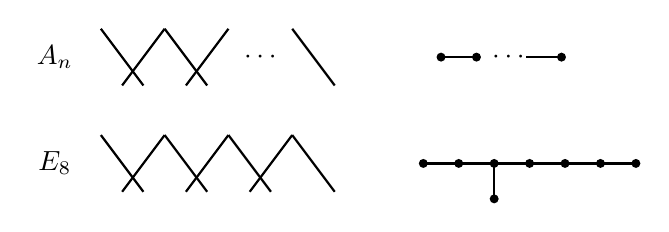
\begin{tikzpicture}[scale=0.9,line width=0.8pt]
  \node at (-0.85,0.55) {$A_n$};
  \draw (-0.2,0.95) -- (0.4,0.15);
  \draw (0.1,0.15) -- (0.7,0.95);
  \draw (0.7,0.95) -- (1.3,0.15);
  \draw (1.0,0.15) -- (1.6,0.95);
  \node at (2.05,0.55) {$\cdots$};
  \draw (2.5,0.95) -- (3.1,0.15);
  \fill (4.6,0.55) circle (1.8pt);
  \draw (4.6,0.55) -- (5.1,0.55);
  \fill (5.1,0.55) circle (1.8pt);
  \node at (5.55,0.55) {$\cdots$};
  \draw (5.8,0.55) -- (6.3,0.55);
  \fill (6.3,0.55) circle (1.8pt);
  \node at (-0.85,-0.95) {$E_8$};
  \draw (-0.2,-0.55) -- (0.4,-1.35);
  \draw (0.1,-1.35) -- (0.7,-0.55);
  \draw (0.7,-0.55) -- (1.3,-1.35);
  \draw (1.0,-1.35) -- (1.6,-0.55);
  \draw (1.6,-0.55) -- (2.2,-1.35);
  \draw (1.9,-1.35) -- (2.5,-0.55);
  \draw (2.5,-0.55) -- (3.1,-1.35);
  \fill (4.35,-0.95) circle (1.8pt);
  \draw (4.35,-0.95) -- (4.85,-0.95);
  \fill (4.85,-0.95) circle (1.8pt);
  \draw (4.85,-0.95) -- (5.35,-0.95);
  \fill (5.35,-0.95) circle (1.8pt);
  \draw (5.35,-0.95) -- (5.85,-0.95);
  \fill (5.85,-0.95) circle (1.8pt);
  \draw (5.85,-0.95) -- (6.35,-0.95);
  \fill (6.35,-0.95) circle (1.8pt);
  \draw (6.35,-0.95) -- (6.85,-0.95);
  \fill (6.85,-0.95) circle (1.8pt);
  \draw (6.85,-0.95) -- (7.35,-0.95);
  \fill (7.35,-0.95) circle (1.8pt);
  \draw (5.35,-0.95) -- (5.35,-1.45);
  \fill (5.35,-1.45) circle (1.8pt);
\end{tikzpicture}
\caption{一些 ADE \trSurface\trSingularPoint{}的解消中的\trExceptionalDivisor，以及它们相应的对偶图（见\mbox{注记~22.4.5}）。（依原书手绘图重绘。）}\label{fig:ade-dynkin}
\end{figure}

\textbf{22.4.6.}\ \emph{\trhRemark{}：\trResolutionOfSingularities。}\quad \trHironaka{}的\trResolutionOfSingularities{}定理蕴含：一般地，「通过胀开\trSingularLocus{}来解消\trSingularPoint」这一想法在\trCharacteristic{} $0$ 下能够成功（见 [Hir] 与 [Ko2]）。（维数 $1$ 的情形将在 \S28.4.4 中证明，维数 $2$ 的情形将在 \S28.6.4 中讨论。）类似的陈述在正\trCharacteristic{}下是否为真尚不可知（维数至多 $3$ 的情形除外；见 [CP]），但\trDeJong{}的\textbf{\trAlterationTheorem}（Alteration Theorem）[dJ] 给出了一个对大多数应用而言足够好的结果：它并不给出从某个正则之物到 $X$ 的\trBirational\trProper{}映射 $\widetilde{X}\to X$，而是给出一个来自某个正则之物的\trProper{}映射，其为一般有限的（并且相应的函数域扩张是可分的）。

下面是一些与\trResolutionOfSingularities{}有关的其他练习。

\textbf{22.4.G.（练习）}\quad 胀开正则概形的一个非既约\trSubscheme{}可能给你带来\trSingular{}之物，本例即是一例。请描述 $\Spec k[x,y]=\mathbb{A}^2$ 中\trClosedSubscheme{} $V(y,x^2)$ 的\trBlowup。证明你得到一个 $A_1$ \trSurface\trSingularPoint。

\textbf{22.4.H.（练习）}\quad 对\trTacnode{}（见\mbox{练习~10.7.G} 与\mbox{定义~28.2.2}）$y^2=x^4$ \trDesingularization：不像\mbox{练习~22.4.D} 那样分两步走，而是一步到位——胀开 $(y,x^2)$。

\textbf{22.4.I.（练习：借一个出乎意料的胀开解消\trSingularPoint）}\quad 设 $Y$ 是\trCone{}面 $x^2+y^2=z^2$，而 $X$ 是 $Y$ 上由 $x=0$、$y=z$ 切出的直线。证明 $\mathrm{Bl}_X\,Y$ 是\trRegular{}的。（此处我们是在胀开一个不是\trEffectiveCartierDivisor{}的余维数 $1$ 轨迹；见\mbox{问题~13.1.3}。但在离开\trCone{}点的地方它是\trEffectiveCartierDivisor，所以你应当预期：你的答案在离开\trCone{}点之处是\trIsomorphism。）

\textbf{22.4.7.}\ \emph{函数在\trRegular{}点处的\trMultiplicity。}\quad 为了提出\mbox{练习~22.4.J}，我们引入一个有用的概念。若 $f$ 是\trLocally\trNoetherian{}\trScheme{} $X$ 上的一个函数，则它在\trRegular{}点 $p$ 处的\textbf{\trMultiplicity}（multiplicity at a regular point），是使 $f$ 落入局部环 $\OO_{X,p}$ 中\trMaximalIdeal{}的 $m$ 次幂之内的最大的 $m$。例如，若 $f\neq 0$，则 $V(f)$ 在 $p$ 处\trSingular{}当且仅当 $m>1$。（你明白这是为什么吗？）

\textbf{22.4.J.（练习）}\quad 证明：在原点处作\trBlowup{}时，$\mathbb{A}^n$ 的\trSubscheme{} $Z$ 的\trTotalTransform{}中\trExceptionalDivisor{}的\trMultiplicity，等于 $Z$ 的一个定义方程（在原点处）的最小\trMultiplicity。（例如，对上面的\trNode{}\trCurve{}与\trCusp{}\trCurve{}的情形，即\mbox{例~22.4.3} 与\mbox{练习~22.4.C}，\trExceptionalDivisor{}都以重数 $2$ 出现。）警示：在着手求解之前，你需要先把这个问题说精确。

\textbf{22.4.8. 解消\trRationalMap。}

\textbf{22.4.K.（练习：借胀开理解\trBirational\trRationalMap{} $\mathbb{P}^2\dashrightarrow\mathbb{P}^1\times\mathbb{P}^1$）}\quad 设 $p$、$q$ 是 $\mathbb{P}^2$ 中两个不同的 $k$-点，并设 $r$ 是 $\mathbb{P}^1\times\mathbb{P}^1$ 的一个 $k$-点。请描述一个\trIsomorphism{} $\mathrm{Bl}_{\{p,q\}}\mathbb{P}^2\overset{\sim}{\longleftrightarrow}\mathrm{Bl}_r\,\mathbb{P}^1\times\mathbb{P}^1$。（可能的提示：考虑过 $p$ 的直线 $\ell$ 与过 $q$ 的直线 $m$；这样一对直线的选取，相应于 $\mathbb{P}^1\times\mathbb{P}^1$ 的一个点。$\mathbb{P}^2$ 中不在直线 $\overline{pq}$ 上的一个点 $s$，给出一对直线 $(\overline{ps},\overline{qs})$，即 $\mathbb{P}^1\times\mathbb{P}^1$ 的一个点。反之，选取一对直线 $(\ell,m)$，只要 $\ell$ 与 $m$ 都不是直线 $\overline{pq}$，便给出一个点 $s=\ell\cap m\in\mathbb{P}^2$。这就描述了一个\trBirational\trRationalMap{} $\mathbb{P}^2\dashrightarrow\mathbb{P}^1\times\mathbb{P}^1$。\mbox{练习~22.4.A} 与此有关。）

\mbox{练习~22.4.K} 是接下来两道练习所探究的那个一般现象的一个例子。

\textbf{22.4.L.（较难而有用的练习：胀开解消到射影空间之\trRationalMap{}的\trBaseLocus）}\quad 设我们有一个\trScheme{} $Y$、一个\trInvertibleSheaf{} $\mathscr{L}$，以及 $\mathscr{L}$ 的若干个\trSection{} $s_0,\dots,s_n$（一个\trLinearSystem，\mbox{定义~15.2.1}）。那么，在由 $s_0=\cdots=s_n=0$ 切出的\trClosedSubscheme{} $X$（该\trLinearSystem{}的\trBaseLocus）之外，这些\trSection{}给出一个到 $\mathbb{P}^n$ 的\trMorphism。证明：这个\trMorphism{}可以唯一地延拓为一个\trMorphism{} $\mathrm{Bl}_X\,Y\to\mathbb{P}^n$，且这个\trMorphism{}相应于\trInvertibleSheaf{} $(\beta^*\mathscr{L})(-\mathrm{E}_X\,Y)$，其中 $\beta\colon\mathrm{Bl}_X\,Y\to Y$ 是\trBlowup{}\trMorphism。换言之：「把概形论\trBaseLocus{}胀开，便解消了这个\trRationalMap」。提示：只须考虑 $Y$ 的一个使 $\mathscr{L}$ 平凡的\trAffine\trOpenSubset{}即可。唯一性或可借用\mbox{练习~11.3.G}。

\textbf{22.4.9.}\ \emph{\trhRemark。}\quad
（i）\mbox{练习~22.4.L} 立即蕴含：胀开可以用来解消到射影概形的\trRationalMap{} $Y\dashrightarrow Z\hookrightarrow\mathbb{P}^n$。

（ii）下面的解读富有启发。$Y$ 上的\trLinearSystem{}拉回为 $\mathrm{Bl}_X\,Y$ 上的\trLinearSystem，而 $Y$ 上\trLinearSystem{}的\trBaseLocus{}拉回为 $\mathrm{Bl}_X\,Y$ 上的\trBaseLocus。$\mathrm{Bl}_X\,Y$ 上的\trBaseLocus{}正是 $\mathrm{E}_X\,Y$，一个\trEffectiveCartierDivisor。由于 $\mathrm{E}_X\,Y$ 不仅\trLocallyPrincipal，而且还局部地是个\trNonZerodivisor，故可以把它从诸 $\beta^*s_i$ 中「除出去」（由此得到 $(\beta^*\mathscr{L})(-\mathrm{E}_X\,Y)$ 的一个\trSection），从而去除\trBaseLocus，留下一个\trBasePointFree{}的\trLinearSystem。（借\trUniversalProperty{}可以把这件事说精确：这是 $Y$ 的能够去除\trBaseLocus{}的最小「修改」。）若 $X$ 本来就是\trCartier{}的（例如，当 $Y$ 是\trRegular{}\trPureDimensional{}\trCurve{}时，任何非平凡的\trLinearSystem{}都必然如此），那么我们只须「把 $X$ 除出去」便能去除\trBaseLocus。

（iii）你或许愿意重访\mbox{练习~19.7.C}，并用\mbox{练习~22.4.L} 的语言来解读它。

\textbf{22.4.10.}\ \emph{若干例子。}\quad
（i）由 $[x_0,\cdots,x_n]\dashrightarrow[x_1,\cdots,x_n]$ 给出、定义在 $p=[1,0,\cdots,0]$ 之外的\trRationalMap{} $\mathbb{P}^n\dashrightarrow\mathbb{P}^{n-1}$，可以通过胀开 $p$ 来解消。于是，由\mbox{\trBlowupClosureLemma~22.2.7}，若 $Y$ 是 $\mathbb{P}^n$ 的任一局部闭\trSubscheme，那么一旦胀开 $Y$ 中的 $p$，我们便可投射到 $\mathbb{P}^{n-1}$，而给出这个到 $\mathbb{P}^{n-1}$ 之映射的\trInvertibleSheaf{}是（稍显不正式地说）$\beta^*(\OO_{\mathbb{P}^n}(1))\otimes\OO(-\mathrm{E}_p\,Y)$。

（ii）考虑三个变元的两个一般齐次三次函数 $C_1$ 与 $C_2$，它们给出 $\mathbb{P}^2$ 中两条三次曲线。二者都\trSmooth{}（由\mbox{\trBertini{}定理~13.4.2}），并相交于九个点 $p_1,\dots,p_9$（利用我们的\trStandingHypothesis：在代数闭域上工作）。于是 $[C_1,C_2]$ 给出一个\trRationalMap{} $\mathbb{P}^2\dashrightarrow\mathbb{P}^1$。为了解消这个\trRationalMap，我们胀开 $p_1,\dots,p_9$。所得结果（一般地）是一个\emph{\trEllipticFibration}（elliptic fibration）$\mathrm{Bl}_{\{p_1,\dots,p_9\}}\mathbb{P}^2\to\mathbb{P}^1$。（这绝算不上一个完整的论证，甚至算不上一个精确的陈述。）

（iii）取定 $\mathbb{P}^2$ 中六个一般的点 $p_1,\dots,p_6$。在这些点上消失的三次函数构成一个四维\trVectorSpace，而且它们恰好概形论地消失且仅消失于这些点。这就给出一个\trRationalMap{} $\mathbb{P}^2\dashrightarrow\mathbb{P}^3$，通过胀开这六个点可以将其解消。所得的\trMorphism{}结果是一个\trClosedEmbedding，而它在 $\mathbb{P}^3$ 中的像是一个（光滑的）三次曲面。这就是那个著名的事实：平面在六个一般点处的胀开可以表示为 $\mathbb{P}^3$ 中的一个（光滑）三次曲面。（同样，这个论证也无意求全。）更精确、更完整的讨论见 \S27.3.5。

在合理的情形下，\mbox{练习~22.4.L} 有一个借\trRationalMap{}之图像的解读。

\textbf{22.4.M.（练习）}\quad 设 $s_0,\dots,s_n$ 是\trIntegral\trScheme{} $X$ 上某个\trInvertibleSheaf{} $\mathscr{L}$ 的\trSection，不全为 $0$。由\mbox{注记~15.2.5}，这些资料给出一个\trRationalMap{} $\phi\colon X\dashrightarrow\mathbb{P}^n$。请在 $\phi$ 的图像（\S11.3.4）与 $\mathrm{Bl}_{V(s_0,\dots,s_n)}\,X$ 之间给出一个\trIsomorphism。（你的论证将不需要在\trField{} $k$ 上工作；它在一般情形下都成立。）

你或许会乐于探究前一个想法，亲手演算一下\trCremona{}变换 $\mathbb{P}^2\dashrightarrow\mathbb{P}^2$（\mbox{练习~7.5.J}）如何能借\trRationalMap{} $[x,y,z]\dashrightarrow[1/x,\,1/y,\,1/z]$ 的图像来解读。

\textbf{22.4.N.}\ \hard\ \textbf{（练习）}\quad 解消从\trQuadricSurface{}上的\trCone{}出发、到射影直线的\trRationalMap
\[
\Spec k[w,x,y,z]/(wz-xy)\mathrel{\overset{[w,x]}{\dashrightarrow}}\mathbb{P}^1.
\]
设 $X$ 是所得的\trVariety，而 $\pi\colon X\to\Spec k[w,x,y,z]/(wz-xy)$ 是到\trQuadricSurface{}上的那个\trCone{}的\trProjection。证明：$\pi$ 在离开\trCone{}点处是\trIsomorphism，且\trCone{}点的原像\trIsomorphic{}于 $\mathbb{P}^1$（从而具有余维数 $2$，故不同于单纯胀开\trCone{}点所得的那个解消）。可能的提示：若 $Q$ 是 $\mathbb{P}^3$ 中由 $wz-xy=0$ 切出的\trQuadricSurface，则把这个\trRationalMap{}分解为 $\Spec k[w,x,y,z]/(wz-xy)\setminus\{0\}\to Q$（参看\mbox{练习~9.3.N}），继以\trIsomorphism{} $Q\overset{\sim}{\longrightarrow}\mathbb{P}^1\times\mathbb{P}^1$（\mbox{例~10.6.2}），再投射到其中一个因子。

这是一个\textbf{\trSmallResolution}（small resolution）的例子。（\trSmallResolution{} $X\to Y$ 是这样一种解消：$Y$ 中纤维具有维数 $r$ 的点的轨迹，其余维数大于 $2r$。我们不会再以任何实质的方式用到这个概念。警示：这是\trIntersectionHomology（intersection homology）中所用的「小解消」定义；在\trMinimalModelProgram{}中，小解消则指在余维数 $1$ 处为\trIsomorphism{}的解消。所以请留意你所读内容的语境。）注意，这个对态射的解消涉及胀开\trBaseLocus{} $w=x=0$，它是以\trQuadricSurface $wz=xy$ 上某条直线为底的\trCone。我们是在胀开一个\trEffective\trWeilDivisor，由于这个胀开不是\trIsomorphism，它必然不是\trCartier{}的。在\mbox{练习~13.1.E} 中我们曾看到 $(w,x)$ 不是\trPrincipal{}的，而这里我们看到 $(w,x)$ 甚至不是\trLocallyPrincipal{}的。本质上由\mbox{练习~15.5.N}，$V(w,x)$ 甚至不能充当任何\trLocallyPrincipal{}除子的\trSupport。

\textbf{22.4.11.}\ \emph{\trhRemark{}：互不同构的小解消。}\quad 如果你改为解消映射 $[w,y]$，你将得到一个看起来相像的小解消
\[
\pi'\colon X'\longrightarrow\Spec k[w,x,y,z]/(wz-xy)
\]
（它在离开原点处是\trIsomorphism，而原点之上的纤维是 $\mathbb{P}^1$）。但它有所不同！更精确地说：不存在使下图交换的\trMorphism{} $X\to X'$\footnote{原书此处作「making the following the diagram commute」，当为「making the following diagram commute」之误，径改。——译者注}
\[
\begin{tikzcd}
X \ar[rr] \ar[dr,"\pi"'] && X' \ar[dl,"\pi'"] \\
& \Spec k[w,x,y,z]/(wz-xy) &
\end{tikzcd}
\]
\trBirational\trRationalMap{} $X\dashrightarrow X'$ 称作\textbf{\trAtiyahFlop}（Atiyah flop），[At1]。

\textbf{22.4.12.}\ \emph{\trBirational\trRationalMap{}的分解。}\quad 在结束关于\trRationalMap{}之解消的讨论之际，我们指出：正如\trHironaka{}定理断言，在\trCharacteristic{} $0$ 下，人们可以沿光滑\trSubvariety{}的\trBlowup{}序列解消\trVariety{}的一切\trSingularPoint（\S22.4.6），\emph{\trWeakFactorizationTheorem}（Weak Factorization Theorem）（首由 Włodarczyk 证明 [Wl]）同样断言：\trCharacteristic{} $0$ 下任意两个\trBirational{}的\trVariety{} $X$ 与 $Y$，都可以借沿光滑\trSubvariety{}的胀开与「收缩」联系起来。更精确地说：存在\trVariety
\[
X_0,\ \dots,\ X_n,\ X_{01},\ \dots,\ X_{(n-1)n}
\]
（其中 $X_0=X$、$X_n=Y$），并存在\trMorphism{} $X_{i(i+1)}\to X_i$ 与 $X_{i(i+1)}\to X_{i+1}$（$0\le i<n$），它们都是光滑\trSubvariety{}的胀开。

\textbf{22.4.13. 胀开与线丛。}

\textbf{22.4.O.（练习：推广\mbox{练习~20.2.D}）}\quad 设 $X$ 是 $k$ 上的一张正则射影曲面，$p$ 是一个 $k$-\trValuedPoint。令 $\beta\colon\mathrm{Bl}_pX\to X$ 为\trBlowup{}\trMorphism，并令 $\mathrm{E}=\mathrm{E}_pX$ 为\trExceptionalDivisor。考虑\eqref{eq:excision-class-groups} 的那个\trExactSequence
\[
\mathbb{Z}\mathrel{\xrightarrow{\ \gamma\colon 1\mapsto[\mathrm{E}]\ }}\mathrm{Pic}(\mathrm{Bl}_pX)\mathrel{\xrightarrow{\ \alpha\ }}\mathrm{Pic}(\mathrm{Bl}_pX\setminus\mathrm{E})\longrightarrow 0
\]
（严格说来，\eqref{eq:excision-class-groups} 中 $\mathrm{Pic}$ 被换成了 $\mathrm{Cl}$。但由于正则局部环都是\trUFD{}（\S13.8.5），依\mbox{命题~15.4.16}，此情形下 $\mathrm{Pic}=\mathrm{Cl}$。）注意 $\mathrm{Bl}_pX\setminus\mathrm{E}=X\setminus p$。证明 $\mathrm{Pic}(X\setminus p)=\mathrm{Pic}\,X$。证明 $\beta^*\colon\mathrm{Pic}\,X\to\mathrm{Pic}\,\mathrm{Bl}_pX$ 给出 $\alpha$ 的一个截面。用 \S22.3.4 证明 $\OO_{\mathrm{Bl}_pX}(\mathrm{E})|_{\mathrm{E}}\cong\OO_{\mathrm{E}}(-1)$\footnote{原书此处作「$\OO_X(E)|_E$」，当为「$\OO_{\mathrm{Bl}_pX}(E)|_E$」之误（$\mathrm{E}$ 是胀开 $\mathrm{Bl}_pX$ 上的除子，本练习下文亦作 $\OO_{\mathrm{Bl}_pX}(\mathrm{E})$），径改。——译者注}（于是，用第 20 章的语言，$\mathrm{E}$ 是一条 $(-1)$-曲线，\mbox{定义~20.2.8}），并由此证明 $\gamma$ 是一个\trInjection。结论：$\mathrm{Pic}\,\mathrm{Bl}_pX\cong\mathrm{Pic}\,X\oplus\mathbb{Z}$。请描述如何由 $\mathrm{N}^1_{\mathbb{Q}}(X)$ 上的相交矩阵求出 $\mathrm{N}^1_{\mathbb{Q}}(\mathrm{Bl}_pX)$ 上的相交矩阵。

\textbf{22.4.P.（练习）}\quad 设 $D$ 是 $X$ 上的一个\trEffectiveCartierDivisor{}（一条\trCurve）。令 $\operatorname{mult}_pD$ 为 $D$ 在 $p$ 处的\trMultiplicity{}（\mbox{练习~22.4.J}），并令 $D^{\mathrm{pr}}$ 为 $D$ 的\trProperTransform。证明：作为\trEffectiveCartierDivisor，有 $\beta^*D=D^{\mathrm{pr}}+(\operatorname{mult}_pD)\mathrm{E}$。更精确地，证明：$D^{\mathrm{pr}}$ 的局部方程与 $\mathrm{E}$ 的局部方程的 $(\operatorname{mult}_pD)$ 次幂二者的乘积，正是 $\beta^*D$ 的局部方程，从而（i）$\beta^*D$ 是一个\trEffectiveCartierDivisor，且（ii）$\beta^*\OO_X(D)\cong\OO_{\mathrm{Bl}_pX}(D^{\mathrm{pr}})\otimes\OO_{\mathrm{Bl}_pX}(\mathrm{E})^{\otimes(\operatorname{mult}_pD)}$。（\mbox{提示~20.2.7} 中的方程 $\ell=e+m$ 便是其一个特例。）

\textbf{22.4.14.}\ \emph{胀开之下典范线丛的变化。}\quad 作为「\trCanonical{}线丛在胀开之下如何变化」的动机，考虑胀开 $\beta\colon\mathrm{Bl}_{(0,0)}\mathbb{A}^2\to\mathbb{A}^2$。为方便计，令 $X=\mathrm{Bl}_{(0,0)}\mathbb{A}^2$、$Y=\mathbb{A}^2$。我们将用\mbox{练习~21.4.A} 来关联 $\beta^*\mathscr{K}_Y$ 与 $\mathscr{K}_X$。

我们在 $(0,0)$ 附近为 $\mathscr{K}_Y$ 选取一个生成元：$\mathrm{d}x\wedge\mathrm{d}y$。（事实上，它在 $\mathbb{A}^2$ 上处处都是 $\mathscr{K}_Y$ 的生成元，但为了便于推广，我们指出：要紧的只是它是 $(0,0)$ 处的生成元，从而由几何\trNakayama{}引理（\mbox{练习~14.3.D}）它也是 $(0,0)$ \emph{附近}的生成元。）把它拉回到 $X$ 上时，我们可以把它解读为 $\mathscr{K}_X$ 的一个\trSection；它将生成 $\mathscr{K}_X$ 在\trExceptionalDivisor{} $\mathrm{E}$ 之外的部分，但可能带着某个重数 $\mu$ 包含 $\mathrm{E}$。回想：$X$ 可以被解读为「$\mathbb{A}^2$ 中的一个点」外加「过原点的一条直线的选取」这份数据。我们考虑直线非竖直的那个\trOpenSubset{} $U$，此时这条直线可以写成 $y=mx$。这里我们有自然的\trCoordinate：$U=\Spec k[x,y,m]/(y-mx)$，我们可以把它解读为 $\Spec k[x,m]$。\trExceptionalDivisor{} $\mathrm{E}$ 与 $U$ 相交于 $x=0$ 处（在 $U$ 的\trCoordinate{}之下），所以我们可以在这些开集上计算 $\mu$。把 $\mathrm{d}x\wedge\mathrm{d}y$ 拉回到 $U$ 上，我们得到
\[
\mathrm{d}x\wedge\mathrm{d}y=\mathrm{d}x\wedge\mathrm{d}(xm)=m(\mathrm{d}x\wedge\mathrm{d}x)+x(\mathrm{d}x\wedge\mathrm{d}m)=x(\mathrm{d}x\wedge\mathrm{d}m)
\]
（因为 $\mathrm{d}x\wedge\mathrm{d}x=0$）。于是 $\beta^*(\mathrm{d}x\wedge\mathrm{d}y)$ 沿 $\mathrm{E}$ 以阶 $1$ 消失。

\textbf{22.4.Q.（练习，参看不重要的\mbox{练习~21.4.J}）}\quad 请解释这一计算如何给出一个\trCanonical\trIsomorphism{} $\mathscr{K}_X\overset{\sim}{\longleftrightarrow}(\beta^*\mathscr{K}_Y)(\mathrm{E})$。

\textbf{22.4.R.（练习）}\quad 在维数 $n$ 的情形重复上面的计算。证明\trExceptionalDivisor{}以重数 $(n-1)$ 出现。

\textbf{22.4.S.}\ \hard\ \textbf{（练习）}\quad 设 $k$ 是\trPerfectField。
（a）设 $Y$ 是 $k$ 上的一张曲面，$p$ 是一个正则的 $k$-\trValuedPoint，并设 $\beta\colon X\to Y$ 是 $Y$ 在 $p$ 处的胀开。证明 $\mathscr{K}_X\cong(\beta^*\mathscr{K}_Y)(\mathrm{E})$。提示：为找 $\mathscr{K}_X$ 在 $p$ 附近的生成元，选取 $\mathfrak{m}/\mathfrak{m}^2$ 的生成元 $\bar{x}$、$\bar{y}$（其中 $\mathfrak{m}$ 是 $\OO_{Y,p}$ 的\trMaximalIdeal），并把它们提升为 $\OO_{X,p}$ 的元素。为什么 $\mathrm{d}x\wedge\mathrm{d}y$ 在 $p$ 处生成 $\mathscr{K}_X$？
（b）在任意维数下重复（a）（依循\mbox{练习~22.4.R}）。
（c）设 $Z$ 是光滑 $n$ 维\trVariety{} $Y$ 的一个光滑 $m$ 维（闭）\trSubvariety，并设 $\beta\colon X\to Y$ 是 $Y$ 沿 $Z$ 的胀开。证明 $\mathscr{K}_X\cong(\beta^*\mathscr{K}_Y)((n-m-1)\mathrm{E})$。（回想\mbox{定理~22.3.10}：$X=\mathrm{Bl}_Z\,Y$ 是\trSmooth{}的。）

\textbf{22.4.15.}\ \hard\ \textbf{\trQuasiprojective\trScheme{}的维数上同调消失（曾于 \S18.2.7 中许诺）。}\quad
借助\trBlowup{}的理论，\mbox{定理~18.2.6}（射影 $k$-\trScheme{}上诸\trQCSheaf{}的维数\trCohomology{}消失）可以被推广到\trQuasiprojective{} $k$-\trScheme。设 $X$ 是维数为 $n$ 的\trQuasiprojective{} $k$-\trVariety。我们将证明 $X$ 可以被 $n+1$ 个仿射开子集覆盖。由于 $X$ \trQuasiprojective，存在某个射影\trVariety{} $Y$ 带一个开嵌入 $X\hookrightarrow Y$。把 $Y$ 换成 $X$ 在 $Y$ 中的闭包后，不妨设 $\dim Y=n$。在 $X$ 于 $Y$ 中的补集上任意放置一个\trSubscheme{}结构 $Z$（例如，\trReduced{}子概形结构，\S9.4.9）。令 $Y'=\mathrm{Bl}_Z\,Y$。则 $Y'$ 是一个射影\trVariety{}（\S22.3.1），可以被 $n+1$ 个仿射开子集覆盖。$X$ 在 $Y'$ 中的补集是一个\trEffectiveCartierDivisor{}（$\mathrm{E}_Z\,Y$），于是由\mbox{练习~8.3.E}，$Y'$ 的这些仿射开子集中每一个限制到 $X$ 上仍是仿射的\footnote{原书此处作「\,$Y$\,的这些仿射开子集」，当为「\,$Y'$\,的这些仿射开子集」之误（前文已令 $Y'=\mathrm{Bl}_Z\,Y$，此处讨论的覆盖属于 $Y'$），径改。——译者注}。

\textbf{22.4.16.}\ \emph{\trhRemark。}\quad
（i）你或许会随即希望：\emph{任何}维数为 $n$ 的\trVariety{}都能被 $n+1$ 个仿射开子集覆盖。这并不成立。对每个整数 $m$，都存在一个至少需要 $m$ 个仿射开集才能覆盖的三维体；见 [RotV, Ex.~4.9]。由上面的讨论可知，这个例子必然不是\trQuasiprojective{}的。
（ii）下面是一条在\trInvariantTheory（invariant theory）中有用的事实，它可以用同样的方式证明。设 $p_1,\dots,p_n$ 是\trQuasiprojective{} $k$-\trVariety{} $X$ 上的\trClosedPoint。那么 $X$ 有一个包含它们全部的仿射开子集。

\textbf{22.4.T.（练习：\trQuasiprojective\trVariety{}的维数上同调消失）}\quad 设 $X$ 是维数为 $d$ 的\trQuasiprojective{} $k$-\trScheme。证明：对 $X$ 上任意一个\trQC{}\trSheaf{} $\mathscr{F}$，当 $i>d$ 时 $\mathrm{H}^i(X,\mathscr{F})=0$。

\textbf{22.4.17.}\ \extrahard\ \textbf{\trDeformationToTheNormalCone（图~\ref{fig:deformation-normal-cone}）。}

\begin{figure}[htbp]
\centering
\begin{tikzpicture}[scale=0.9,line width=0.8pt]
  \draw (0,4.35) rectangle (6.6,5.5);
  \draw[gray!60,line width=0.6pt] (0.55,4.35) -- (0.55,5.5);
  \draw[gray!60,line width=0.6pt] (1.1,4.35) -- (1.1,5.5);
  \draw[gray!60,line width=0.6pt] (1.65,4.35) -- (1.65,5.5);
  \draw[gray!60,line width=0.6pt] (5.1,4.35) -- (5.1,5.5);
  \draw[gray!60,line width=0.6pt] (5.6,4.35) -- (5.6,5.5);
  \draw[gray!60,line width=0.6pt] (6.1,4.35) -- (6.1,5.5);
  \node at (0.28,4.95) {$Y$};
  \node at (0.83,4.95) {$Y$};
  \node at (5.35,4.95) {$Y$};
  \node at (5.85,4.95) {$Y$};
  \draw[dotted,line width=0.9pt] (3.3,5.5) .. controls (3.15,5.28) and (3.28,5.12) .. (3.22,4.98);
  \draw (3.22,4.98) .. controls (3.1,4.82) and (3.18,4.64) .. (3.28,4.52);
  \draw (3.28,4.52) -- (3.52,4.66);
  \draw (3.28,4.52) -- (3.52,4.38);
  \draw[->] (4,4.52) -- (3.58,4.52);
  \node at (4.5,4.52) {$\mathrm{N}_X\,Y$};
  \draw[gray!75,->] (3.3,4.25) -- (3.3,3.4);
  \draw (0,2.15) rectangle (6.6,3.3);
  \draw[gray!60,line width=0.6pt] (0.55,2.15) -- (0.55,3.3);
  \draw[gray!60,line width=0.6pt] (1.1,2.15) -- (1.1,3.3);
  \draw[gray!60,line width=0.6pt] (1.65,2.15) -- (1.65,3.3);
  \draw[gray!60,line width=0.6pt] (5.1,2.15) -- (5.1,3.3);
  \draw[gray!60,line width=0.6pt] (5.6,2.15) -- (5.6,3.3);
  \draw[gray!60,line width=0.6pt] (6.1,2.15) -- (6.1,3.3);
  \draw (3.3,3.3) -- (3.3,2.9) .. controls (3.02,2.74) and (3.02,2.56) .. (3.28,2.42);
  \draw (3.28,2.42) -- (3.52,2.57);
  \draw (3.28,2.42) -- (3.52,2.27);
  \draw[->] (3.95,3.02) -- (3.45,3.02);
  \node at (4.55,3.02) {$\mathrm{Bl}_X\,Y$};
  \draw[->] (2.62,2.66) -- (3.12,2.66);
  \node at (2.15,2.66) {$\mathrm{E}_X\,Y$};
  \draw[->] (3.98,2.34) -- (3.58,2.34);
  \node at (4.55,2.34) {$\mathrm{N}_X\,Y$};
  \draw[gray!75,->] (3.3,2.05) -- (3.3,1.22);
  \node at (3.05,1.64) {$\beta$};
  \draw (0,0) rectangle (6.6,1.15);
  \draw[gray!60,line width=0.6pt] (0.55,0) -- (0.55,1.15);
  \draw[gray!60,line width=0.6pt] (1.1,0) -- (1.1,1.15);
  \draw[gray!60,line width=0.6pt] (1.65,0) -- (1.65,1.15);
  \draw[gray!60,line width=0.6pt] (5.1,0) -- (5.1,1.15);
  \draw[gray!60,line width=0.6pt] (5.6,0) -- (5.6,1.15);
  \draw[gray!60,line width=0.6pt] (6.1,0) -- (6.1,1.15);
  \draw[line width=1.1pt] (3.3,1.15) -- (3.3,0.55);
  \fill (3.3,0.55) circle (2pt);
  \node at (3.58,0.55) {$X$};
  \draw[gray!75,->] (3.3,-0.07) -- (3.3,-0.5);
  \node at (-1.05,1.35) {$Y$};
  \draw (-1.05,1.15) -- (-1.05,0.15);
  \fill (-1.05,0.15) circle (2pt);
  \node at (-0.78,0.15) {$X$};
  \draw (0,-0.62) -- (7.2,-0.62);
  \fill (3.3,-0.62) circle (2pt);
  \node at (3.3,-0.92) {$0$};
  \node at (7.55,-0.62) {$\mathbb{A}^1$};
  \draw[gray!75,->] (6.7,2.6) .. controls (7.9,1.7) and (7.6,0.1) .. (6.95,-0.58);
  \draw[gray!75,->] (6.7,0.6) .. controls (7.5,0.15) and (7.3,-0.35) .. (6.6,-0.6);
  \node at (7.25,1.65) {$\pi$};
  \node[align=center] at (8.6,3.7) {\emph{到\trNormal\trCone}\\ \emph{的形变}};
\end{tikzpicture}
\caption{\trDeformationToTheNormalCone（\S22.4.17）。（依原书手绘图重绘。）}\label{fig:deformation-normal-cone}
\end{figure}

下面这个构造，是现代理解代数几何中相交理论（正如 Fulton 与 MacPherson 所发展的那样，[F2]）的关键。

\textbf{22.4.U.（练习：\trDeformationToTheNormalCone）}\quad 设 $Y$ 是一个 $k$-\trVariety，而 $X\hookrightarrow Y$ 是一个\trClosedSubscheme。
（a）证明 $\beta\colon\mathrm{Bl}_{X\times 0}(Y\times\mathbb{A}^1)\to Y\times\mathbb{A}^1$ 的\trExceptionalDivisor{}\trIsomorphic{}于 $X$ 在 $Y$ 中的\trNormal\trCone{}的射影完备化。
（b）设 $\pi\colon\mathrm{Bl}_{X\times 0}(Y\times\mathbb{A}^1)\to\mathbb{A}^1$ 是 $\beta$ 与到 $\mathbb{A}^1$ 的\trProjection{}的\trComposition。证明：$\pi^{-1}(0)$ 是 $\mathrm{Bl}_X\,Y$ 与 $X$ 在 $Y$ 中的\trNormal\trCone{}的射影完备化二者的概形论并，而这两个\trSubscheme{}的交可以与 $\mathrm{E}_X\,Y$ 等同起来——后者以通常的方式（作为胀开 $\mathrm{Bl}_X\,Y\to Y$ 的\trExceptionalDivisor）是 $\mathrm{Bl}_X\,Y$ 的一个\trClosedSubscheme，并且是\trNormal\trCone{}之射影完备化的一个\trClosedSubscheme，如\mbox{练习~9.3.O} 所描述的那样。

映射
\[
\mathrm{Bl}_{X\times 0}(Y\times\mathbb{A}^1)\setminus\mathrm{Bl}_X\,Y\longrightarrow\mathbb{A}^1
\]
称作\textbf{\trDeformationToTheNormalCone}（deformation to the normal cone）（「$Y$ 到 $X$ 在 $Y$ 中的\trNormal\trCone{}的形变」之简称）。注意：对 $\mathbb{A}^1$ 中远离 $0$ 的每个 $k$-点，其上方的纤维都\trCanonically{}\trIsomorphic{}于 $Y$，而 $0$ 上方的纤维是\trNormal\trCone。由于这个\trFamily{}「和善」（更精确地说，平坦——这是第 24 章的论题），我们便可以经由这个退化来证明关于一般 $Y$（在 $X$ 附近）的一些事情。（我们将在 \S24.3.10 中看到，\trDeformationToTheNormalCone{}是一个平坦\trMorphism，这在相交理论中很有用。）

